\documentclass[12pt]{article}\usepackage[]{graphicx}\usepackage[]{color}
%% maxwidth is the original width if it is less than linewidth
%% otherwise use linewidth (to make sure the graphics do not exceed the margin)
\makeatletter
\def\maxwidth{ %
	\ifdim\Gin@nat@width>\linewidth
	\linewidth
	\else
	\Gin@nat@width
	\fi
}
\makeatother

\definecolor{fgcolor}{rgb}{0.345, 0.345, 0.345}
\newcommand{\hlnum}[1]{\textcolor[rgb]{0.686,0.059,0.569}{#1}}%
\newcommand{\hlstr}[1]{\textcolor[rgb]{0.192,0.494,0.8}{#1}}%
\newcommand{\hlcom}[1]{\textcolor[rgb]{0.678,0.584,0.686}{\textit{#1}}}%
\newcommand{\hlopt}[1]{\textcolor[rgb]{0,0,0}{#1}}%
\newcommand{\hlstd}[1]{\textcolor[rgb]{0.345,0.345,0.345}{#1}}%
\newcommand{\hlkwa}[1]{\textcolor[rgb]{0.161,0.373,0.58}{\textbf{#1}}}%
\newcommand{\hlkwb}[1]{\textcolor[rgb]{0.69,0.353,0.396}{#1}}%
\newcommand{\hlkwc}[1]{\textcolor[rgb]{0.333,0.667,0.333}{#1}}%
\newcommand{\hlkwd}[1]{\textcolor[rgb]{0.7te37,0.353,0.396}{\textbf{#1}}}%

%\usepackage{framed}
%\makeatletter
%\newenvironment{kframe}{%
%	\def\at@end@of@kframe{}%
%	\ifinner\ifhmode%
%	\def\at@end@of@kframe{\end{minipage}}%
%\begin{minipage}{\columnwidth}%
%	\fi\fi%
%	\def\FrameCommand##1{\hskip\@totalleftmargin \hskip-\fboxsep
%		\colorbox{shadecolor}{##1}\hskip-\fboxsep
%		% There is no \\@totalrightmargin, so:
%		\hskip-\linewidth \hskip-\@totalleftmargin \hskip\columnwidth}%
%	\MakeFramed {\advance\hsize-\width
%		\@totalleftmargin\z@ \linewidth\hsize
%		\@setminipage}}%
%{\par\unskip\endMakeFramed%
%	\at@end@of@kframe}
%\makeatother

\definecolor{shadecolor}{rgb}{.97, .97, .97}
\definecolor{messagecolor}{rgb}{0, 0, 0}
\definecolor{warningcolor}{rgb}{1, 0, 1}
\definecolor{errorcolor}{rgb}{1, 0, 0}
\newenvironment{knitrout}{}{} % an empty environment to be redefined in TeX

\usepackage{alltt} % use larger type; default would be 10pt

\usepackage[T5]{fontenc}
\usepackage[utf8]{inputenc} % set input encoding (not needed with XeLaTeX)

%%% Examples of Article customizations
% These packages are optional, depending whether you want the features they provide.
% See the LaTeX Companion or other references for full information.

%%% PAGE DIMENSIONS
\usepackage{geometry} % to change the page dimensions
\geometry{letterpaper} % or letterpaper (US) or a5paper or....
\geometry{margin=1.2in} % for example, change the margins to 2 inches all round
% \geometry{landscape} % set up the page for landscape
%   read geometry.pdf for detailed page layout information

\usepackage{graphicx} % support the \includegraphics command and options

% \usepackage[parfill]{parskip} % Activate to begin paragraphs with an empty line rather than an indent

%%% PACKAGES
\usepackage{booktabs} % for much better looking tables
\usepackage{array} % for better arrays (eg matrices) in maths
\usepackage{paralist} % very flexible & customisable lists (eg. enumerate/itemize, etc.)
\usepackage{verbatim} % adds environment for commenting out blocks of text & for better verbatim
\usepackage{subcaption} % make it possible to include more than one captioned figure/table in a single float
\usepackage{float}
\usepackage{setspace}
\usepackage{pdflscape}
\usepackage{amsmath}
\usepackage{url}
\usepackage{multirow}
\usepackage{listings}
\usepackage{dcolumn}
%\usepackage[nolists]{endfloat}
\usepackage{bbm}
\usepackage{pdflscape}
\usepackage{pdfpages}

\usepackage{natbib}
\bibliographystyle{apsr}
\usepackage{hyperref}

\usepackage{tikz} 
\usetikzlibrary{arrows,decorations.pathmorphing,decorations.pathreplacing,backgrounds,fit,positioning,shapes.symbols,chains}

%%% HEADERS & FOOTERS
\usepackage{fancyhdr} % This should be set AFTER setting up the page geometry
\pagestyle{fancy} % options: empty , plain , fancy
\renewcommand{\headrulewidth}{0pt} % customise the layout...
\lhead{}\chead{}\rhead{}
\lfoot{}\cfoot{\thepage}\rfoot{}

%%% SECTION TITLE APPEARANCE
\usepackage{sectsty}
\allsectionsfont{\sffamily\mdseries\upshape} % (See the fntguide.pdf for font help)
% (This matches ConTeXt defaults)

%%% ToC (table of contents) APPEARANCE
\usepackage[nottoc,notlof,notlot]{tocbibind} % Put the bibliography in the ToC
\usepackage[titles,subfigure]{tocloft} % Alter the style of the Table of Contents
\renewcommand{\cftsecfont}{\rmfamily\mdseries\upshape}
\renewcommand{\cftsecpagefont}{\rmfamily\mdseries\upshape} % No bold!

%%% Some commands
\newcommand{\reg}{\texttt{regress} }
\newcommand{\1}{\mathbbm{1}}

\renewcommand\r{\right}
\renewcommand\l{\left}
\newcommand\E{\mathbbm{E}}
\newcommand\V{\mathbbm{V}}
\newcommand\Var{\mathbbm{V}}
\newcommand\avar{{\rm Avar}}
\newcommand\dist{\buildrel\rm d\over\sim}
\newcommand\iid{\stackrel{\rm i.i.d.}{\sim}}
\newcommand\ind{\stackrel{\rm indep.}{\sim}}
\newcommand\cov{{\rm Cov}}
\newcommand{\R}{\textbf{R} }
\newcommand{\Rcmd}[1]{{\large \texttt{#1}}}
\newcommand\indep{\protect\mathpalette{\protect\independenT}{\perp}}
\def\independenT#1#2{\mathrel{\rlap{$#1#2$}\mkern2mu{#1#2}}}
\DeclareMathOperator{\sgn}{sgn}
\DeclareMathOperator*{\argmin}{argmin}

\newcommand\Sum{\sum^N_{i=1}}
\newcommand\Prod{\prod^N_{i=1}}
\newcommand{\pderiv}[1]{\frac{\partial}{\partial #1}}
\newcommand{\B}[1]{\boldsymbol{#1}}
\newcommand{\logit}{\text{logit}}

%opening
\title{Vietnam's Tea Leaf Elections: \\
	Inferring Purpose for Authoritarian Elections from Post-election Responses to Local Defeats}
\author{Minh Trinh}



\begin{document}

\maketitle

\begin{abstract}
	
%The literature on authoritarian elections has often suggested that authoritarian regimes may use elections as an information-gathering device, but has not agreed on which information exactly these regimes are gathering from elections. I argue that authoritarian leaders limit themselves to seeking from elections  only some specific piece of information but not others to avoid receiving conflicting signals from the same election. Furthermore, it is possible to use authoritarian regimes’ response to unexpected electoral upsets to infer what kind of information they are seeking, and then use this knowledge to infer their purpose for authoritarian elections. I demonstrate this logic by analyzing the Communist Party of Vietnam's (CPV) responses to defeats by regime-favored candidates for the national legislature. The analysis identifies a positive causal effect of electoral defeats on central transfers and public goods investment, suggesting that the CPV increased transfers and investment to placate unhappy voters in places they suffered defeats in. Given the context of Vietnam, this pattern of behavior corroborate the view that the CPV uses authoritarian elections to collect information about the geographic distribution of public support for the regime.
\end{abstract}

\doublespacing

\section{Introduction}

%An explanation for why authoritarian regimes choose to hold elections is that authoritarian elections may bring to dictators many benefits that outweigh the risk and cost of holding them. One particular benefit of authoritarian elections is information, which can be acquired by studying patterns of electoral returns across constituencies. The literature, however, has arrived at no consensus about what specific information authoritarian regimes seek to infer from elections. More critically, theories about information flow from authoritarian elections have failed to recognize that election results can be interpreted in multiple ways, among those some may be contradictory to others. How authoritarian leaders choose between competing interpretations of the same election result may shed light on their intention for holding elections. I focus in particular on the ``geographic distribution'' theory, which suggests that authoritarian leaders use elections to infer the geographic distribution of regime support in subnational units, and the ``local bureaucrats'' theory, which suggests that they use elections to monitor government officials in the same units, and seek to find out which theory applies in the context of the elections for the National Assembly in Vietnam, a situation when only one could hold true.
%
%I analyze the responses by the central government in Vietnam -- led by the Communist Party of Vietnam (CPV) -- to the defeats of candidates nominated by the central government (versus candidates nominated by local governments) in three legislative elections in 2007, 2011 and 2016 to identify which of these two theories describes better the party's interpretation of election results and its motive for holding elections. I focus in particular on adjustments to central transfers from the central government to individual provinces. Because central transfers are wholly determined by the country's highest leadership, it is a good proxy to study the regime's decisions. I argue that the ``geographic distribution'' theory would predict that the central government perceives defeats of central nominees as evidence of fledging popularity in specific provinces, and responds by increasing central transfers to these provinces in order to placate the public. On the other hand, the ``local bureaucrats'' theory would predict that it sees these defeats as signaling incompetence and/or disloyalty on the part of provincial bureaucrats who are in charge of managing elections, and thus decreases central transfers to the same provinces to punish these bureaucrats. Adjudicating between these two theories thus requires identifying the causal effect of election defeats on central transfers to provinces. To accomplish this goal, I employ linear fixed-effects regressions over an appropriate subset of the data to achieve identification, and rely on randomization inference to conduct finite-sample tests of the main hypotheses. Additional analyses using the synthetic control method provide robustness checks.
%
%My analysis shows that the CPV generally responds to electoral upsets by increasing transfers to the provinces where defeats occurred. This pattern of response would be expected in a regime that uses elections to gather information on the geographic distribution of regime support. Through its empirical findings, this paper contributes to literature by demonstrating an approach to test competing theories of authoritarian elections. It also highlights the potential for discord between these theories, which could go unnoticed when theory-building advances too far ahead of theory-testing. The findings also suggest that authoritarian regimes may prefer to use elections as a tool for bottom-up rather than top-down accountability, in the sense that they rely on election results to appropriately respond to public dissatisfaction rather than to punish under-performing bureaucrats. Although this shows that authoritarian regimes are capable of meeting public dissatisfaction with concessions, it also echoes the literature's other findings that seemingly democratic institutions may end up reinforcing the durability of authoritarianism \citep[e.g.][]{BoixSvolik2013, GandhiPrzeworski2007}.
%
%The paper begins in section \ref{sec:info} by reviewing the literature on the ``information flow'' theories of authoritarianism. As part of the review, the paper draws attention to the two potentially contradictory theories of ``geographic distribution'' and ``local bureaucrats.'' Then, in section \ref{sec:vietnam}, I provide information about the National Assembly election in Vietnam, and suggest how the Vietnam case could be used to test these two theories. Section \ref{sec:methods} then discusses my empirical approaches, and section \ref{sec:results} summarizes the results. Section \ref{sec:conclusion} reviews the results and their implications, then finally concludes.


\section{The informational limits of authoritarian elections}
\label{sec:info}
To explain why authoritarian regimes choose to hold elections that they may not always win, the literature on authoritarian elections have proposed that these elections may bring certain benefits to those who hold it, arguing that dictators rationally accept the risk of holding elections to secure these benefits. Thus existing theories have argued that authoritarian leaders uses elections as a platform for power-sharing, providing non-violent means for elites to contest over patronage \citep{LustOkar2006} or for dissidents to express dissatisfaction \citep{AR2005}. Elections are also said to help divide and conquer the opposition and co-opt some of them into the regime \citep{LustOkar2005}, or as a ``show of strength'' for the regime to impress upon its opponents the invulnerability of its rule and futility of resistance \citep{Geddes2005}. 

In addition to these explanations, a substantial literature on the ``information flow'' theories of authoritarian institutions\footnote{I borrowed this term from \cite{Hou2017}} has found that authoritarian regimes use nominally democratic institutions to gather various kinds of information to aid them in their rules. These theories have great potential for explaining the purpose of authoritarian elections: elections and the results they generate do indeed generate a lot of information that a calculating dictator may utilize. \cite{Geddes2005} for instance suggests that authoritarian regimes can look at election results to know how popular or strong their opposition is. Elaborating on this line of reasoning, \cite{Miller2015} finds that autocratic regimes use elections to estimate citizen dissatisfaction with the regime. The logic is that because the ruling party in an autocratic regime can ensure that voting against it would incur significant but not categorically unbearable personal costs to citizens, voters would only dare to do so when they are genuinely dissatisfied. Negative election results, in particular electoral shocks, thus credibly communicate the true level of dissatisfaction, allowing the ruling regime to respond to public needs only when necessary. An even more nuanced argument suggests that the variation in election results across constituencies sheds light not on the general \textit{level}, but on the sub-national \textit{distribution} of regime popularity. Autocratic leaders can then use this information to identify opposition strongholds to suppress \citep{Magaloni2006, Blaydes2008} or marginal districts to buy off \citep{Reed2001, Magaloni2006}. Additionally, election results also convey information about the competence or loyalty of individual agents within the regime machinery, in particular the government bureaucrats tasked with managing the elections and delivering results on behalf of the regime \citep{Magaloni2006, Blaydes2008, Myagkov2009, RundlettSvolik2016}. Finally, unexpectedly strong performance by regime outsiders can also alert the regimes to potential threats, or indicate for them which elites should be co-opted into the regime \cite{LustOkar2005}.

HERE I NEED TO OFFER MY OWN THEORY

Even as each of these theories is built upon solid theoretical and empirical work, it may not be possible for all of them to simultaneously hold true. The reason is that an election cannot accomplish an intended objective on its own, but requires some engineering or manipulation on the part of the dictator before it can credibly deliver overwhelming victories, reveal pockets of dissidents, highlight competent regime agents, etc. While a dictator may truly hold an election with multiple objectives in mind, as soon as manipulating an election to pursue an objective makes it less suitable for another objective, it becomes unreasonable for this dictator to expect the election to fulfill both. In other words, a particular autocrat cannot use a particular to achieve \textit{all} the goals the literature thinks it can \textit{at the same time}, because optimizing an election to achieve one goal makes it harder to achieve at least one another. For instance, for an election to effectively demonstrate the strength of a regime, its leaders must manipulate the electoral process such that the final results show overwhelming support for ruling party. In doing so, however, the regime makes it less likely that these results would reveal any pocket of resistance, or that any potential outsider would even stand for, let alone stand out in, such a manipulated election. As a result, the demonstration objective directly undermines the information objective of the election. This implies that a rational dictator would not use the same election to both demonstrate its strength and to gather information about its opponents; the two corresponding theories (\cite{Geddes2005} and \cite{LustOkar2005}) thus cannot simultaneously hold.

This same argument holds particularly for the ``information flow'' theories of elections. To understand this line of reasoning, consider that, even without any external action by the regime, the output of an election only becomes information after it has been interpreted by the regime leaders. Election results are after all raw numbers; for them to imply anything about the level of regime support, the existence of potential challengers, or the conduct of election officials, a connection must somehow be drawn between the numbers and these often unobserved quantities. The dictator makes this connection by attempting to interpret election results in terms of these quantities. An interpretation in this sense is an explanation, or more precisely a causal attribution that links the observed results with unobserved phenomena, established through a process not unlike how campaign officials in democracies interpret the electoral performance of their candidates/parties.\footnote{To argue that individuals ``interpret'' election results they have may seem like attributing to them hyper-rationality, but the actual ``interpretation'' may simply be an attempt to attribute blame for defeats or credit for victories, which may benefit from but does not require much cognitive sophistication from each individual.} In other words, what information the authoritarian regime can draw from an election is intrinsically tied to how it explains to itself the observed election results.

Multiple potential interpretations \textit{may} exist for any set of election results, but objectively only one \textit{can} truly apply. A humiliating defeat for the regime may be caused, for example, by either unenthusiastic regime agents failing to manipulate the process hard enough, by a frustrated public feeling disillusioned enough to accept the risk of voting against the regime, or most likely by a weighted mixture of these causes. An unlimited number of such mixture can theoretically generate the same set of election results: imagine, for instance, an alternate reality in which the regime agents are slightly more zealous in their duty, only to be perfectly offset by a slightly more fearful public. In reality, however, only one mixture of variables -- one that did in fact manifest on election day -- could be said to truly have caused cause the observed election results. In other words, the underlying causes behind a set of election results are as unique and unchanging as the observed results. 

The dictator's own interpretation of the observed election results, on the other hand, is only an attempt at guessing these unchanging causes. This is never an easy task. It is also consequential, because guessing the wrong cause leads to the wrong information being generated and the wrong lessons being learned. How, then, can dictators ensure that they can draw correct information from elections? One practical approach is to manipulate each election in such a way that neutralizes most alternative determinants of election results, leaving only those variables that they care about. By placing rigid controls on the electoral processes' moving parts, not only do authoritarian regimes increase their chance of winning, but they also shrink the set of potential explanations behind election results to those factors uncontrolled for. As an example, banning opposition parties or candidates ensures that vote shares for the incumbents are not influenced by support for the opposition. As another example, forcing all candidates to run in districts they are not local in eliminates personal popularity as an explanation for every candidate's performance. In this sense, an authoritarian regime's ``menu of manipulation'' \citep{Schedler2002menu} may also serve to refine the information that authoritarian elections may generate.

Authoritarian regimes vary in how effectively they manage the uncertainty of elections, but all of them become vulnerable to learning the wrong lesson the moment they seek to multitask. The reason is that, for elections to shed light on any variable, this variable needs to be kept somewhat unmanaged, such that it still has some influence over election results. A regime seeking to learn multiple kinds of information from an election thus has to keep multiple variables unmanaged, giving up certainty in exchange for information. Between multiple unmanaged variables, however, exists infinite possible mixtures, multiple of which could theoretically explain why an election turned out the way it did. As long as the regime cannot identify which exact mixture of these many variables is responsible for the observed results, there is no way for it to know how much the results are indicative of one underlying phenomenon versus another, leaving it constantly at risk of attributing too much on one cause and too little on the other.\footnote{In statistical lingo, the ruling party is unable to point-identify how much each factor contributes to the bad result. To achieve point-identification it may be necessary to hold one factor constant or ignorable, for example by using randomization. Most readers would agree though that it is unreasonable to expect that politicians always see and behave like social scientists.}  As a result, dictators who seek to learn multiple kinds of information from one election remain unsure about what information they end up receiving. Rational dictators are therefore unlikely to seek different types of information from the elections they hold.

Authoritarian regimes may also refrain from using elections to collect multiple types of information if their repertoire of post-election responses is so limited that two different interpretations for a same set of results would inform two contradictory courses of action. To understand this argument, note that if authoritarian regimes were to use elections as sources of information as the ``information flow'' theories suggest, we should expect these regimes to make adjustments to policies immediately upon the observation of certain election results. Following this logic, a regime seeking to infer multiple types of information from the same election should be expected to make multiple different adjustments to different policies upon observing the same results. In certain cases, however, the number of policy instruments that the regime can adjust in response to incoming information from elections may be limited. This is true for regimes with limited capacity, since their lack of capacity means they have fewer levers to pull in any circumstance, not just in post-election contexts. But high-capacity regimes may also encounter this kind of limits if these regimes have such highly structured institutions that there is little discretion in policy adjustments in the period immediately following elections. Single-party or military regimes fit particularly well this description , and so do federal or similarly hierarchical regimes.\footnote{Multiple typologies of authoritarian regimes exist in the literature \citep[see, for instance,][]{GeddesWrightFrantz2014, Wahman2013}. Here I am relying primarily on the classification by \citet{GeddesWrightFrantz2014}}.

For any regime, as long as it seeks different types of information from elections, a single set of election results may generate different pieces of information, which in turn recommend as responses different policy adjustments. Even with unrestricted response options, the regime still needs to decide or allocate weights among different pieces of informations, which then requires them to decide or allocate weights among various policy responses. In response to a humiliating defeat, for instance, the regime may decide to punish its agents or voters depending on whether it believes their own agents' failing or the voters defiance lie at the root of the regime's defeat. Because the regime cannot know how much of the defeat can be blamed on incompetent agents and how much on dissenting voters, it cannot decide how much punishment to throw upon its agents and how much on voters.

When the authoritarian regime's repertoire of post-election responses is limited, it becomes more likely that the response to one piece of information would compromise the response to the other piece of information. In the above example, punishing regime agents may turn out to benefit disobedient citizens by helping them get rid of incongruent officials, whereas suppressing voters may end up giving more power to regime agents. In this case, wrongly allocating weights between different interpretations of election results may cause both post-election responses to backfire. Because distinguishing between different interpretations becomes harder when the regime seeks a wide range of information from elections, for regimes with limited options for post-election responses, intending to collect too many types of information from elections only increases the probability that post-election responses are counter-productive. For these regimes, as long as the regime leaders are adequately rational, it is even more unlikely that they would hold elections for multiple different informational purposes. 

In summary, authoritarian regimes should rationally refrain from collecting multiple types of information from elections, because doing so would complicate these regimes' ability to learn the correct lesson from any election result, and this problem only worsens for regimes with limited options for post-election responses. This argument has some important implications for the literature. Because authoritarian regimes in general and authoritarian regimes with limited post-election policy instruments in particular are expected to avoid seeking multiple types of information from elections, it is only logical that not every ``information flow'' theories of elections, each of which positing a different purpose for authoritarian elections, can all apply to the same election. In other words, even as each theory among the many ``information flow'' theories can credibly explain the purpose behind those elections that theory is built upon, when generalizing beyond those cases to identify the intention behind hitherto unexplained elections, care should be taken to adjudicate between these different theories. 

Adjudicating between different ``information flow'' theories matters more than just for determining the relative intellectual merits of each theory. Firstly, each of these theories has different implications for the state of accountability in the country cases studied. Where elections help inform autocrats about the loyalty of their agents instead of the mood of the citizenry, top-down accountability can be said to thrive over bottom-up accountability. Conversely, when dictators use elections to evaluate its popularity among voters, voters can credibly use the ballots to express their feelings towards the ruling regime's policies, convincing the regime to adjust policies even when election results do not result in turnovers. Less optimistically, when dictators use elections only to achieve spectacular victories, little can be expected of voters' ability to use their ballots to make regime leaders respond to their needs and demands. Knowing which, if any, form of accountability exists in an authoritarian country helps guide efforts in studying the politics of this country, directing scholars towards actors that matter more, and to interactions that determine a greater share of political outcomes in that country. 

Secondly, this knowledge also informs evaluation about the prospect of democratization or liberalization of the country. Where elections help citizens hold regime leaders accountable, democratic norms may take hold easily. Conversely, where elections serve only as yet another tool for autocrats to police their followers, it is hard to imagine these autocrats feeling vulnerable enough to relinquish powers to the public. 

Finally, the literature may benefit from truly testing theories of authoritarian elections \textit{vis-\`{a}-vis} another. Existing works have only considered a small subset of theories at once, and have not conducted many comparative evaluation between pairs of theories to identify which theory fits better with empirical evidence. The one-country case studies that dominate this literature \citep{LustOkar2005, Geddes2005, Magaloni2006, Blaydes2008} often devote more effort proposing new theories rather than testing old ones. The result is an abundance of claims about what information authoritarian regimes seek from elections, but no clear conclusion about which claim carries the most weight. For understanding of authoritarian elections to advance, it is necessary to both explore more explicitly the conditions that make some theories more plausible than others, and subject these theories to more rigorous tests under these conditions.
 
%The same argument holds to a lesser but still considerable extent for the ``information flow'' theories of elections. On one hand, it is entirely possible for an election to generate different kinds of information, and reasonable for regime leaders to look for all of them in the same election. Since autocrats only have to passively observe the electoral process and the resulting vote counts to receive information from an election, they do not face the same conundrum as in the above case, where one action they take to help the election achieve one objective would necessarily compromise another. In other words, conditional on a level of manipulation, an election can tell the regime as much about public opinion as it does about regime agents or potential political rivals. On the other hand, the true process that goes on in an election and produces its result is often unknown. A particular defeat of a regime-favored candidate, for instance, can either be caused by overwhelming public dissatisfaction with the regime, or personal failings of that candidate. Regime leaders, having only , only the final vote counts to rely on, must exercise an act of interpretation to explain to themselves why an election turns out the way it does. This act of interpretation is especially crucial when different explanations of an election result would suggest different follow-up actions: a regime-favored candidate who lost because of his own failings should face punishment, but one who loses because of general public disillusion with the regime should not. For a regime to decide on which course of action to take, it must therefore limit the number of interpretations it can have of an election result, which then implies that the regime can see from this election only a subset of the information it can generate. In other words, in most cases, an authoritarian regime may only seek some information but not others from elections, meaning that not all ``information flow'' theories can apply to explain its actions.

\subsection{Local defeats help adjudicate between theories of authoritarian elections}
\label{sec:local_defeat}

It is possible to extend the ``information flow'' theories to argue that authoritarian elections are the most informative when they result in \textit{some} upsets for the regime. Under authoritarian regimes, electoral upsets are rarely expected but never impossible, even when the ruling regimes possess a ``menu of manipulation'' \citep{Schedler2002menu}. In particular, parliamentary elections under authoritarian regimes do sometimes lead to \textit{local defeats} -- defeats by regime candidates in local constituencies they run in. 

Local defeats are often a result of ambitious and innovative strategies by the opposition \citep{BunceWolchik2010} or certain regime weaknesses \citep{LevistkyWay2010}, but even in the case of dominant- or single-party regimes where competition is muffled \citep{Schedler2002} and the regime is strong \citep{BunceWolchik2010}, local defeats may still happen even if much less frequently. To begin with, authoritarian leaders may be aware that election fraud diminishes the informational value of elections \citep{Wintrobe2000}, and thus volunteer to refrain from excessive fraud on election day. Instead they may choose to tilt the playing field through pre-election manipulation of electoral institutions \citep{DiazMagaloni2001, Pepinsky2009, MaleskySchuler2011}, which reduces but does not eliminate the risk of losing for some of the regime's candidates. Additionally, competition under dominant- or single-party regimes also takes place more vigorously along alternative cleavages like the center-periphery divide. Indeed, even when all the candidates compete under the same party banner, some of them may still represent local interests that run counter to that of the central party leadership. Such conflict of interest exists even in extremely institutionalized single-party regimes like China \citep{Manion2014} or Vietnam \citep{MaleskySchuler2011}. For these regimes, victories by candidates representing the peripheral interests over those representing the central interests in local constituencies can be considered local defeats.
	
Since authoritarian regimes rarely suffer and thus do not expect unsatisfactory results, any defeat would provide a data point so different from their informational prior that dictators can tell it contains more signal than noise. Indeed, whereas a large part of variation in vote share can be attributed to random noise or idiosyncratic factors, only a true aberration could lead to a regime vote share low enough to produce a defeat. Thus, if a regime is truly using elections as a source of information, it should always pay attention to any instance of local defeat, perhaps even more than to vote share \textit{per se}.

It follows further that if an authoritarian regime uses elections as a source of information, because local defeats are high-information events they should be followed by some significant action. Indeed, because every ``information flow'' theory rests on the premise that authoritarian leaders collect information from elections \textit{to calibrate their actions}, it is natural to expect that the large amount of information from local defeats will trigger a behavioral change. Furthermore, we only need to assume that authoritarian regimes prefer winning over losing to believe that they would do something to avoid future repetition of these defeats. 

In either case, as argued above, a regime's post-election response should be informed by the information they have collected. More specifically, how the regime interprets the defeats will influence its thinking about who or what is responsible for the defeats, and consequently which actions should be done to whom to rectify the situation. Figure \ref{fig:Theory} lists for each prevalent theory of authoritarian elections the implied purpose for holding elections, the interpretation of election defeats that corresponds to each purpose, and then the post-election response that logically follows. Not every theory predicts a post-election response to local defeats: according to the ``power-sharing'' theories, local defeats are expected and accepted by-products of elections, and should happen for the offer of power-sharing to be credible \citep{AR2005, Cox2009}. Other theories, such as the co-optation theory \citep{LustOkar2005}, predict post-election responses even if information is not the primary motive for elections. For the ``information flow'' theories, however, post-election responses are not directly predicted but should be expected as a necessary auxiliary outcome: what good is \textit{information} if it does not help \textit{inform} behaviors?

The leverage for testing theories of authoritarian elections come from the possibility that, within specific contexts, regime leaders observing local defeats and interpreting them in a certain way would come up with post-election responses that are counterproductive to those responses they would have come up if they were to interpret these defeats in another way. In this case, for the regime to come up with any response at all, it is necessary that it does not entertain both interpretations. In then follows that at least one theory is not applicable to the case. Not every pair of theories is prone to such incompatibility: each of \cite{Miller2015} and \cite{Geddes2005}, for example, predicts responses that very likely to fit with the other's theory. Many other theories, however, do predict conflicting post-election responses. Between these theories appropriate adjudication can be achieved by observing which of the incompatible predictions ends up occurring. Because behaviors are honest and credible reflection of the dictator's thinking process, looking at which response gets chosen reveals the thinking process triggered in the dictator's mind upon observation of election defeats, and hence the theory that best explains why this dictator held elections in the first place.

HERE I NEED TO MAKE IT CLEARER THAT THIS IS MY THEORY

\section{Adjudicating between two theories of authoritarian elections using Vietnam's National Assembly Elections}

In the above section, I argued that theories of authoritarian elections, especially the ``information flow'' theories that suggest autocrats hold elections for information purpose, are unlikely to apply simultaneously to the same cases, and that looking at post-election responses to local defeats by dictators can reveal the kind of information they obtain from election results, and hence the original information purpose behind holding elections. In this section, I demonstrate this logic by looking at the Vietnamese government's response to a certain kind of election defeats to adjudicate between two popular theories of authoritarian elections. Both these theories are viable at a first glance, but because they imply contradictory post-election results, cannot both apply to the Vietnam case.

\subsection{``Geographic distribution'' vs. ``local bureaucrats''}
Among the ``information flow'' theories, two are particularly at risk of diametrically contradicting each other. One theory suggests that election results provide information on the geographic distribution of support and dissent (henceforth the ``geographic distribution'' theory), whereas the other suggests that election results reveal individual local level party bureaucrats' level of competence or even level of loyalty to the central leadership (henceforth the ``local bureaucrats'' theory). At the same time, they are often given equal spotlight together without acknowledgment of potential conflict, for example in the two seminal works of \cite{Magaloni2006} and \cite{Blaydes2008}. 

Specifically, both scholars posit that electoral results provide information about the geographic distribution of support and dissent for the ruling regime. In Mexico, \cite{Magaloni2006} finds that areas where the ruling PRI captured a greater vote share were deemed as centers of government support, whereas areas with low PRI vote shares were considered opposition strongholds. Similarly, for Egypt, \cite{Blaydes2008} remarks that “election results provide the regime with a map of areas of political support for the opposition.” In both cases, the two authoritarian governments were able to know which sub-national units have higher or lower concentration of regime supporters by looking at where they received a higher or lower vote share. In Mexico, the PRI used this information to reward their supporters, whereas in Egypt the regime instituted a “punishment regime” in opposition strongholds by withholding their public goods investment.

In parallel, both \cite{Magaloni2006} and \cite{Blaydes2008} also suggest that election results provide information about the competence and loyalty of lower-level party members. In both countries, the task of mobilizing voters on behalf of the ruling party is delegated to lower-level party agents, with the national level playing little to no direct role. These agents are not candidates themselves, but play important role in making sure that the ruling party’s candidates get elected. Election results, reflected through turnout as well as through the ruling party' share of the votes, are then perceived as a function of how well these sub-national party members do their job. \cite{Blaydes2008} notes further that a failure to deliver good results may also be a symptom of disloyalty, for example when a local party member forgoes careerist goals within the ruling party to pursue short-term material gains offered by the local opposition candidates by mobilizing on behalf of the opposition instead.\footnote{In Mexico, \cite{Larreguy2016} show that the PRI also extends this method of evaluation to assess the vote-buying performance of local brokers.}

Although each of these two theories of authoritarian elections makes sense on its own, neither \cite{Magaloni2006} nor \cite{Blaydes2008} acknowledge fully that they can be incompatible within one single case. From the perspective of the authoritarian leaders, the level of popular support in a province and the level of competence or loyalty of the party bureaucrats in the same province are two different narratives explaining a same outcome at the same level of disaggregation. Thus, when explaining an electoral upset in a certain province, the first theory would suggest that regime leaders attribute the defeat to the lack of supporters in this province, but the second would suggest they attribute it to the bureaucrats 
the election there. It may be suggested that both theories hold true and the regime believes in both narratives, but even then it remains impossible for the regime to appropriately divide blame attribution for the defeat on these distinct causes.

\begin{figure}[H]

\centering
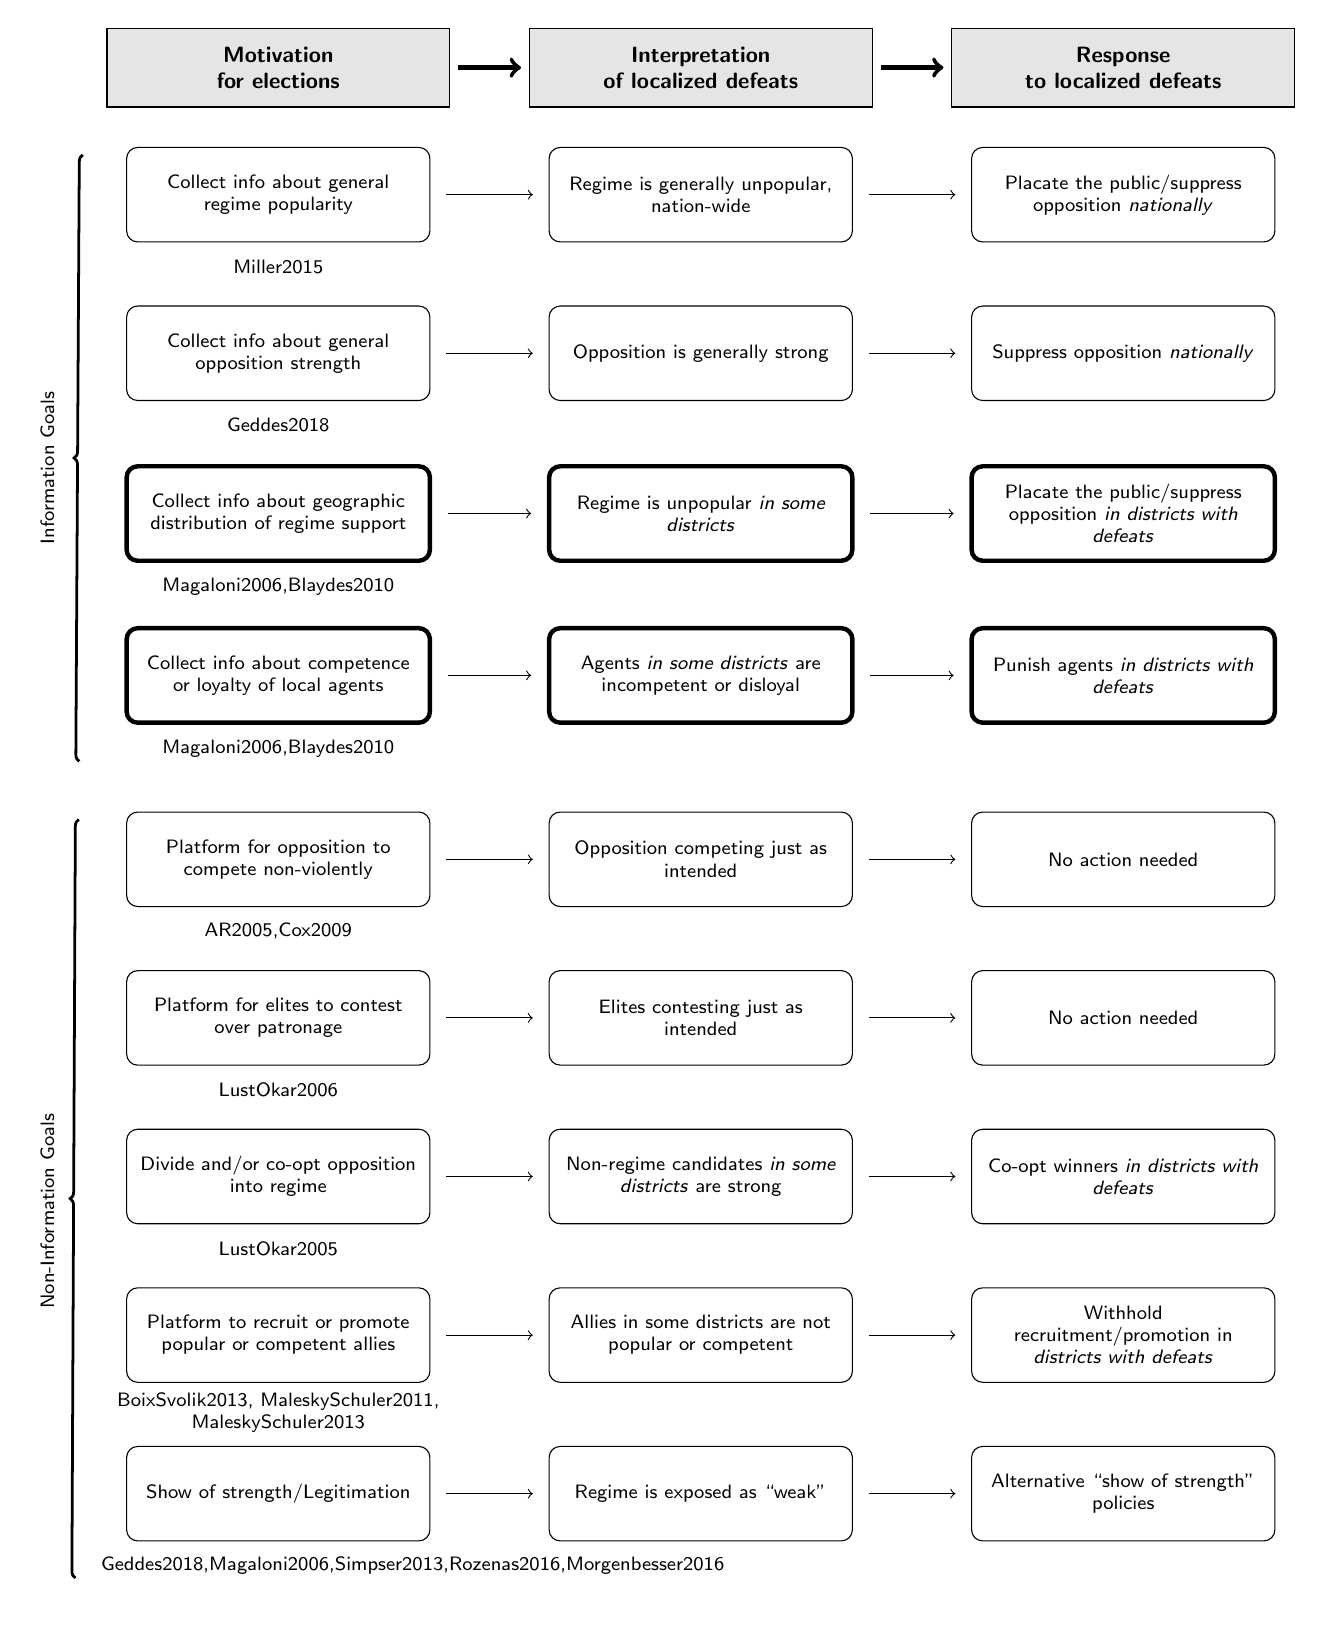
\begin{tikzpicture}
[node distance = 1cm, auto,font=\footnotesize,
% STYLES
every node/.style={node distance=3cm},
% The title style is used to draw the main title
title/.style={rectangle, draw, fill=black!10, inner sep=5pt, text width=4cm, text badly centered, minimum height=1cm, font=\bfseries\footnotesize\sffamily},
% The subtitle style is used to draw the title below main title
subtitle/.style={rectangle, inner sep= 2pt, minimum height=.5cm, node distance=0.25cm, text width=4.5cm, text badly centered, font=\scriptsize\sffamily},
% The theory style is used to draw nodes for each theory
theory/.style={rectangle, rounded corners, draw, minimum height=1.2cm, inner sep= 5pt, text width=3.5cm, node distance=0.25cm, text badly centered, font=\scriptsize\sffamily}]

%%%% Top nodes %%%%
\node [title] (interpretation) {Interpretation\\of localized defeats};
\node [title, left=1cm of interpretation] (intention) {Motivation\\for elections};
\node [title, right=1cm of interpretation] (response) {Response\\to localized defeats};

%% Top nodes subtitle

% Intention
%\node [subtitle, below=0.2cm of intention] (sub-intention) {for\\
%	authoritarian elections};

% Interpretation
%\node [subtitle, below=0.2cm of interpretation] (sub-interpretation) {of\\
%	localized defeats};

% Response
%\node [subtitle, below=0.2cm of response] (sub-response) {to\\
%	localized defeats};

%%%% Theory nodes %%%%
% B1
\node [theory, below=0.5cm of intention] (B1-intention) {Collect info about general regime popularity};
\node [subtitle, below=0.05cm of B1-intention] (B1-sub-intention) {\citep{Miller2015}};

\node [theory, below=0.5cm of interpretation] (B1-interpretation) {Regime is generally unpopular, nation-wide};
\node [subtitle, below=0.05cm of B1-interpretation] (B1-sub-interpretation) {};

\node [theory, below=0.5cm of response] (B1-response) {Placate the public/suppress opposition \textsl{nationally}};
\node [subtitle, below=0.05cm of B1-response] (B1-sub-response) {};

% B2
\node [theory, below=0.8cm of B1-intention] (B2-intention) {Collect info about general opposition strength};
\node [subtitle, below=0.05cm of B2-intention] (B2-sub-intention) {\citep{Geddes2018}};

\node [theory, below=0.8cm of B1-interpretation] (B2-interpretation) {Opposition is generally strong};
\node [subtitle, below=0.05cm of B2-interpretation] (B2-sub-interpretation) {};

\node [theory, below=0.8cm of B1-response] (B2-response) {Suppress opposition \textsl{nationally}};
\node [subtitle, below=0.05cm of B2-response] (B2-sub-response) {};

% B3
\node [theory, below=0.8cm of B2-intention, ultra thick] (B3-intention) {Collect info about geographic distribution of regime support};
\node [subtitle, below=0.05cm of B3-intention] (B3-sub-intention) {\citep{Magaloni2006,Blaydes2010}};

\node [theory, below=0.8cm of B2-interpretation, ultra thick] (B3-interpretation) {Regime is unpopular \textsl{in some districts}};
\node [subtitle, below=0.05cm of B3-interpretation] (B3-sub-interpretation) {};

\node [theory, below=0.8cm of B2-response, ultra thick] (B3-response) {Placate the public/suppress opposition \textsl{in districts with defeats}};
\node [subtitle, below=0.05cm of B3-response] (B3-sub-response) {};

% B4
\node [theory, below=0.8cm of B3-intention, ultra thick] (B4-intention) {Collect info about competence or loyalty of local agents};
\node [subtitle, below=0.05cm of B4-intention] (B4-sub-intention) {\citep{Magaloni2006,Blaydes2010}};

\node [theory, below=0.8cm of B3-interpretation, ultra thick] (B4-interpretation) {Agents \textsl{in some districts} are incompetent or disloyal};
\node [subtitle, below=0.05cm of B4-interpretation] (B4-sub-interpretation) {};

\node [theory, below=0.8cm of B3-response, ultra thick] (B4-response) {Punish agents \textsl{in districts with defeats}};
\node [subtitle, below=0.05cm of B4-response] (B4-sub-response) {};

% A1
\node [theory, below=1.1cm of B4-intention] (A1-intention) {Platform for opposition to compete non-violently};
\node [subtitle, below=0.05cm of A1-intention] (A1-sub-intention) {\citep{AR2005,Cox2009}};

\node [theory, below=1.1cm of B4-interpretation] (A1-interpretation) {Opposition competing just as intended};
\node [subtitle, below=0.05cm of A1-interpretation] (A1-sub-interpretation) {};

\node [theory, below=1.1cm of B4-response] (A1-response) {No action needed};
\node [subtitle, below=0.05cm of A1-response] (A1-sub-response) {};

% A2
\node [theory, below=0.8cm of A1-intention] (A2-intention) {Platform for elites to contest over patronage};
\node [subtitle, below=0.05cm of A2-intention] (A2-sub-intention) {\citep{LustOkar2006}};

\node [theory, below=0.8cm of A1-interpretation] (A2-interpretation) {Elites contesting just as intended};
\node [subtitle, below=0.05cm of A2-interpretation] (A2-sub-interpretation) {};

\node [theory, below=0.8cm of A1-response] (A2-response) {No action needed};
\node [subtitle, below=0.05cm of A2-response] (A2-sub-response) {};

% C1
\node [theory, below=0.8cm of A2-intention] (C1-intention) {Divide and/or co-opt opposition into regime};
\node [subtitle, below=0.05cm of C1-intention] (C1-sub-intention) {\citep{LustOkar2005}};

\node [theory, below=0.8cm of A2-interpretation] (C1-interpretation) {Non-regime candidates \textsl{in some districts} are strong};
\node [subtitle, below=0.05cm of C1-interpretation] (C1-sub-interpretation) {};

\node [theory, below=0.8cm of A2-response] (C1-response) {Co-opt winners \textsl{in districts with defeats}};
\node [subtitle, below=0.05cm of C1-response] (C1-sub-response) {};

% C2
\node [theory, below=0.8cm of C1-intention] (C2-intention) {Platform to recruit or promote popular or competent allies};
\node [subtitle, below=0.05cm of C2-intention] (C2-sub-intention) {\citep{BoixSvolik2013, MaleskySchuler2011, MaleskySchuler2013}};

\node [theory, below=0.8cm of C1-interpretation] (C2-interpretation) {Allies in some districts are not popular or competent};
\node [subtitle, below=0.05cm of C2-interpretation] (C2-sub-interpretation) {};

\node [theory, below=0.8cm of C1-response] (C2-response) {Withhold recruitment/promotion in \textit{districts with defeats}};
\node [subtitle, below=0.05cm of C2-response] (C2-sub-response) {};

% D1
\node [theory, below=0.8cm of C2-intention] (D1-intention) {Show of strength/Legitimation};
\node [subtitle, below=0.05cm of D1-intention] (D1-sub-intention) {\citep{Geddes2018,Magaloni2006,Simpser2013,Rozenas2016,Morgenbesser2016}};

\node [theory, below=0.8cm of C2-interpretation] (D1-interpretation) {Regime is exposed as ``weak''};
\node [subtitle, below=0.05cm of D1-interpretation] (D1-sub-interpretation) {};

\node [theory, below=0.8cm of C2-response] (D1-response) {Alternative ``show of strength'' policies};
\node [subtitle, below=0.05cm of D1-response] (D1-sub-response) {};

%%%% Side theory category nodes %%%%

% B
\node [subtitle, left=1cm of B1-intention.north west, rotate=90, text width = 8cm] (information) {Information Goals};

\draw [decorate,decoration=brace, line width=1pt] 
([xshift=-0.2cm, yshift=0.1cm]B4-sub-intention.south west) -- ([xshift=-0.55cm, yshift=-0.1cm]B1-intention.north west);

% A, C and D together
\node [subtitle, left=1cm of A1-intention.north west, rotate=90, text width = 10cm] (non-information) {Non-Information Goals};

\draw [decorate,decoration=brace, line width=1pt] 
([xshift=-0.25cm, yshift=0.1cm]D1-sub-intention.south west) -- ([xshift=-0.6cm, yshift=-0.1cm]A1-intention.north west);

%% A
%\node [subtitle, left=0.6cm of A1-intention.north west, rotate=90, text width = 4.4cm] (power-sharing) {``Platform''/``Power-sharing''};
%
%\draw [decorate,decoration=brace, line width=1pt] 
%([xshift=-0.2cm, yshift=0.1cm]A2-sub-intention.south west) -- ([xshift=-0.2cm, yshift=-0.1cm]A1-intention.north west);
%
%% C
%\node [subtitle, left=0.6cm of C1-intention.north west, rotate=90, text width = 1.9cm] (co-optation) {``Co-optation''};
%
%\draw [decorate,decoration=brace, line width=1pt] 
%([xshift=-0.2cm, yshift=0.1cm]C2-sub-intention.south west) -- ([xshift=-0.2cm, yshift=-0.1cm]C1-intention.north west);
%
%% D
%\node [subtitle, left=0.6cm of D1-intention.north west, rotate=90, text width = 2cm] (show-of-strength) {``Demonstration''};
%
%\draw [decorate,decoration=brace, line width=1pt] 
%([xshift=-0.2cm, yshift=0.1cm]D1-sub-intention.south west) -- ([xshift=-0.2cm, yshift=-0.1cm]D1-intention.north west);


%%%%%%%%%%%%%%%%

% Draw the links between forces
\path[->,ultra thick, shorten >=.1cm, shorten <=.1cm] 
(intention) edge (interpretation)
(interpretation) edge (response);

\path[->, shorten >=.2cm, shorten <=.2cm] 
(A1-intention) edge (A1-interpretation)
(A1-interpretation) edge (A1-response);

\path[->, shorten >=.2cm, shorten <=.2cm] 
(A2-intention) edge (A2-interpretation)
(A2-interpretation) edge (A2-response);

\path[->, shorten >=.2cm, shorten <=.2cm] 
(B1-intention) edge (B1-interpretation)
(B1-interpretation) edge (B1-response);

\path[->, shorten >=.2cm, shorten <=.2cm] 
(B2-intention) edge (B2-interpretation)
(B2-interpretation) edge (B2-response);

\path[->, shorten >=.2cm, shorten <=.2cm] 
(B3-intention) edge (B3-interpretation)
(B3-interpretation) edge (B3-response);

\path[->, shorten >=.2cm, shorten <=.2cm] 
(B4-intention) edge (B4-interpretation)
(B4-interpretation) edge (B4-response);

\path[->, shorten >=.2cm, shorten <=.2cm] 
(C1-intention) edge (C1-interpretation)
(C1-interpretation) edge (C1-response);

\path[->, shorten >=.2cm, shorten <=.2cm] 
(C2-intention) edge (C2-interpretation)
(C2-interpretation) edge (C2-response);

\path[->, shorten >=.2cm, shorten <=.2cm] 
(D1-intention) edge (D1-interpretation)
(D1-interpretation) edge (D1-response);


\end{tikzpicture} 
\caption{Key theories of authoritarian elections and their predictions about how regime leaders perceive and respond to localized defeats. Two theories most relevant to the Vietnam case are highlighted with bold borders.}
\label{fig:Theory}
\end{figure}


\subsection{Authoritarian Elections in Vietnam}
\label{sec:vietnam}
To test whether leaders in strong authoritarian regimes prefer to use elections to learn about the geographic distribution of regime support or about individual party bureaucrats, this paper will make use of Vietnam as a test case. Vietnam is a single-party state with a strong Communist party, and thus should be a representative case for most theories about institutionalized single-party states. In addition, the high level of control the Communist Party of Vietnam (CPV) has over elections \citep{MaleskySchuler2011} means that local defeats are rare, and that defeats that did happen are more likely to be signal than noise. Finally, in Vietnam many of the top leaders in its 63 provinces are outsiders appointed by the central leadership, but day-to-day government affairs at lower levels are conducted by officials who are often native to the locality they serve in.\footnote{The distinction between two types of government bureaucrats is closely linked to the distinction between ``deployed'' and ``delegated'' bureaucrats made by \cite{Soifer2015} in his study of state-building in Latin America} This means that the CPV faces two monitoring problems that may not be combined: on one hand it needs to monitor the performance of top provincial leaders, but on the other hand it also needs to keep track of the public in each province and its level of support for the regime, which due to potential self-interested information filtering by lower levels of government may not be directly ``legible'' \cite[in the words of][]{Scott1998} to the party leaders in Hanoi. In other words, the CPV has needs for both information about public support at the local level and about local bureaucrats, which makes Vietnam a balanced testing ground for the two theories.

I focus my analysis on the 2016 election for the Vietnamese National Assembly (VNA), the highest legislative body in the country's political system. The 2016 election is not only the most recent, but is also the only election for which sufficient data is available for analysis. Most specifically, only for this election are vote shares data made available for both election winners as well as losers.

\subsubsection{Elections in Vietnam}

\cite{MaleskySchuler2011}, among others \citep[e.g][]{Gainsborough2005}, have described in details the nomination and election process for the VNA. The VNA elections in Vietnam follow an absolute-majority voting system with multiple winners, in which each district can have 3 to 6 candidates running for 2 to 4 seats and voters get to vote for as many candidates as there are seats in the district. District magnitude and number of candidates are determined prior to the election based on population sizes, and follow a fixed formula: a 6-candidate district is allowed 4 seats, a 5-candidate district is allowed 3 seats, and a 4-candidate district is allowed 2 seats.\footnote{A new type of district with 3 candidates with 2 allowed seats was recently introduced for the 2011 election, but has been discontinued by the 2016 election.} In all districts, candidates with the most votes win, as long as their number of votes exceeds 50 percent of registered voters. This form of voting obscures the informational value of vote margins, as one candidate's margin over another also depends on the performance of that other candidate \textit{vis-\`{a}-vis} another.

The key dynamics of the VNA elections, however, take place not on election day, but in the nomination process that precedes it. In this process, before each election, the central party leadership in the outgoing VNA, which is organized as the VNA standing committee (VNASC), draws up a structure for what the incoming NA should look like. The structure takes the form of composition along demographic, political, and functional lines; for instance, the planned structure for the 500-delegate VNA in the 2007 election called for 150 women, 90 members of ethnic minorities, 160 incumbents, 70 under-40 delegates, and 50 non-party members  \citep[506]{MaleskySchuler2011}. Then, through three rounds of \textit{hiệp thương} (negotiation), the central party leadership and provincial institutions put together a list of candidates to fill the slots, and assign them to districts in ways that would best guarantee that the elected VNA follows the planned structure. This is done by first determining quotas breaking down how many candidates of a certain demographic each province (and then each district) should elect, and then ``stuff'' the districts with candidates from this same demographic. For instance, a district the regime expects to elect a lawyer would be contested only by lawyers, a district it expects to elect a member from an ethnic minority would include only candidates from ethnic minorities, etc. As a result, even though within a district individual candidates may compete against each other to gain votes, the aggregate structure of the VNA can be guaranteed. Additionally, even when the CPV allows independent and self-nominated candidates to contest elections, the nomination process also acts a filter to ensure that only those who follow closely the party line are allowed to run.

A central feature of this nomination process is the difference between central and local nominees. Central nominees are candidates who are nominated in the three \textit{hiệp thương} rounds by central party and government institutions, as well as by the national bodies of party front mass organizations. In practice these central nominees are high-ranking party members with important roles in the party or the government, current VNA committee members, or national leaders of these mass organizations. Local nominees, on the other hand, are nominated by provincial level party and government branches as well as by local chapters of the same organizations. During the \textit{hiệp thương} rounds, central candidates are assigned to individual districts, where they will run against local nominees coming from the local province. Central nominees comprise roughly a third of the planned VNA structure, and all of them are expected to win seats. According to \cite{MaleskySchuler2011}, the CPV ensures this outcome by tilting the playing field \textit{ex ante} rather than through election-day manipulation. In particular, they assign these central nominees not to their home districts or districts they have previously served, but to districts where they can win more easily i.e. districts with the more favorable 5-to-3 candidate-to-seat ratio. In addition,  central nominees generally are not assigned to run against each other. Finally, provincial officials are instructed to support these candidates, both by nominating and assigning  weaker candidates to run against them, as well as by running voter education and mobilization campaigns to encourage voters to vote for them. \footnote{\cite{MaleskySchuler2011} show that the CPV eschews \textit{ex post} fraud in favor of \textit{ex ante} electioneering, by conducting digit tests on official results from the 2007 election fail to reject the hypothesis of naturally generated numbers. However, this evidence would only rule out fraud at the highest level but fail to detect manipulation at lower level, as aggregates of manipulated numbers would exhibit patterns similar to the natural generation process. Indeed, interviews with neighborhood-level officials in charge of managing the 2016 election suggest that agents at several polling stations tampered with the tabulation of result. There is however no smoking-gun evidence that such tampering is systematic or ordered by higher levels of government.}

\subsection{``Geographic distribution'' and ``local bureaucrats'': Plausible explanations for local defeats}

Thanks to this sophisticated array of manipulation techniques, the CPV has always managed to maintain a tight control over election results. As \cite{MaleskySchuler2011} show, the party is confident enough in its ability to control election results to set out very specific plans for the structure of the to-be-elected NA, and the near-identity between planned and the actually elected NA shows that its confidence is well warranted. However, the fact that the final result detracts slightly from the plan suggests that the CPV's control is not perfect. Indeed, in all  three most recent elections, there have always been central nominees who suffered unexpected defeats, even though they never comprised more than 15 percent of all the running central nominees: 21 out of 165 for 2007, 14 out of 173 for 2011, and 16 out of 197 for 2016. Their defeats were surprising and important enough to be covered by the state-controlled media \citep[e.g][]{vov2016, laodong2016}.

For the central leadership of the CPV, understanding and interpreting the local defeats of their central nominees is not necessarily straightforward. Careful engineering of the election process has expectedly restricted the space of possible explanations for these defeats, but both an explanation based on the distribution of support and one based on the performance of individual local bureaucrats remain plausible. First of all, local defeats could reflect the geographic distribution of support for the CPV, in the sense that the party commands lower support in provinces that suffered central nominee defeats. This interpretation is valid if voters indeed have some agency to communicate disapproval of the regime through their votes. In Vietnam, this is likely to hold true if voters can recognize central nominees from the ballot and identify them as representatives of the party, and consciously see voting against these nominees as casting a vote of no confidence against the central government. 

Both these conditions are indeed conceivable. The first condition holds because central nominees rarely come from or have worked in the province they run in, and are thus strangers to voters. This contrasts them with local nominees, who most likely would have spent their entire careers in the province. Additionally, as part of the election process in Vietnam, neighborhood-level officials carry out an intense voter education and mobilization campaign, which includes visiting individual households to inform voters of the candidates' profiles, as well as conveying ``suggestions'' about which candidates to vote for. This ensures that voters have plenty of cues, if not about which candidates are central nominees, then about which candidates the government truly prefers. 

The second condition -- that voters see the election as a vote of confidence and cross out central nominees' names to express dissatisfaction towards the regime -- cannot be directly verified, but my interviews both formal and informal with voters in Hanoi and Ho Chi Minh City suggest that a number of them do exhibit exactly this kind of behavior. In particular, some voters comment that they crossed out the names of whoever the neighborhood official suggests to them, whereas some others voted only for independent candidates. In this sense, door-to-door voter education actually emphasized the link between central nominees and the central government, thus providing voters with targets to direct their disapproval. Furthermore, interviews suggest that voters in Vietnam have high confidence that their ballots are kept secret, but also low confidence that they are tabulated correctly. These two beliefs are not contradictory: on the contrary, voters think their ballots are kept secret \textit{precisely because} they believe the regime will not even look at them, choosing instead to make up results in the tabulation process. This means that some voters see voting as an inconsequential act of expression, and do so freely without fear of retribution when dissatisfied. In the end, these voters may have underestimated their efficacy: where voters cast more of such ``protest votes,'' central nominees may end up losing elections despite the biases in their favor.

While it is plausible that local defeats reflect the geographic distribution of support for the CPV, it is no less conceivable that they are the result of weak performance by provincial bureaucrats. This explanation of local defeats emphasizes the capacity of provincial officials to influence election outcomes, as well as a potential conflict of interest between provincial and national leaders. In terms of capacity, it is true that the central party leadership delegates most of the election management power to provincial officials, including the freedom to nominate local candidates to run in their provinces and to allocate the candidates running in their province to electoral districts. Provincial leaders can therefore reduce competition for central nominees by stacking them up against weaker local candidates, or by placing them in districts with more favorable candidate-to-seat ratios. This indeed is a common practice \cite[provided confirmatory evidence for the 2007 election, which I replicated successfully for the 2011 and 2016 elections]{MaleskySchuler2011}.  Additionally, through the infrastructure of the state, local officials can have significant power to directly influence the vote choice of the voters. The door-to-door voter education and mobilization campaign carried out at every neighborhood is a example. If the majority of voters are passive and/or apathetic compliers -- instead of active ``protest voters'' as described above -- then provincial officials can definitely influence election results just by selecting who they tell voters to vote for. Finally, provincial officials can also interfere with the tabulation of results such that the candidates they prefer receive favorable vote shares regardless, even when such local-level manipulation may not be in the best interest of the central government. 

Even though they have a high capacity to influence election outcomes, provincial officials also face a conflict of interest when doing so. On one hand, the central party leadership expects provincial officials to deliver election results that follow the planned structure and that give seats to all central nominees. On the other hand, the provinces also have vested interest in ensuring as many of their candidates as possible make it to the VNA, since these local nominees are either local leaders in the provinces, or representatives of local interests. Although top provincial leaders are appointed by the central government and are often not native to the province they work in, the long tenure of 4-5 years makes it attractive for them to align with the province's interests. Center-periphery divide arises because each elected central nominee takes one seat away from local candidates. Indeed, in 2016, the municipality of Hanoi reportedly demands to have fewer centrally nominated candidates to make room for its own candidates \citep{vnexpress2016_2}. Occasionally, strong central nominees can cost the province even more than one seat. In particular, when central candidates secure too many of the district's votes, the chance that some local candidates may not make it pass the 50 percent threshold increases. When this happens, the district may not be able to elect as many candidates as there are seats alloted for them -- as happened in two provinces in 2016 \citep{vnexpress2016}. As consequence, even when the province genuinely wishes to promote the central nominees, doing so too enthusiastically may end up costing it a representative in the VNA. This means that local officials operate within the boundary of divergent preferences: while the center prefers provinces to devote as much resource as \textit{possible} to the promotion of central nominees, provincial leaders only seek to do so as much as \textit{necessary} to avoid hurting their own candidates. In the ideal scenario, this produces a result acceptable to the center, but when the local officials are too eager to support their own candidates, or too incompetent to exercise their power effectively, central nominees are at risk of losing to local candidates.

\subsection{``Placate'' and ``Punish'': Incompatible post-election responses}
\label{sec:vs}
Without further evidence, both explanations for local defeats seem equally plausible: provinces where central nominees lost could be those where the CPV experienced lower popularity, or those where provincial bureaucrats did a worse job managing the elections. Objectively, the real cause of local defeats is likely a combination of them factors. Most importantly, the ``geographic distribution'' and ``local bureaucrats'' theories are incompatible in Vietnam, because it is not possible for the CPV to act on both interpretations at the same time. As previously argued, each theory of authoritarian elections posits a different intention for holding elections, which determines the interpretation the regime settles on to explain the defeats, and then the post-election responses it carries out after. Seeing elections as generating multiple kinds of information means that the regime has to consider multiple interpretations of the defeat and contemplate multiple courses of actions, with no way to correctly allocate priorities among them. If the courses of action are incompatible i.e. they cannot be pursued simultaneously without one undermining the efficacy of another, then holding multiple interpretations of the defeat leaves the regime in a quandary. In this way, the two explanations for local defeat, and hence the two theories of authoritarian elections, are incompatible not in an objective sense, but only because they predict incompatible actions by the authoritarian regime. This incompatibility is particularly stark in the case of Vietnam, as the two post-election courses of action predicted by each theory would turn out to be diametrically opposite.

If the ``geographic distribution'' theory holds, the regime would see local defeats as indicators for provinces with faltering public support. The appropriate post-action response would be to  \textit{increase} central transfers to these provinces to \textit{placate} the public. In Vietnam, because most provinces spend more money than it can generate through taxes, central transfers are indispensable for public goods provision. Increasing central transfers thus enables increased spending on public goods and other popular programs, which is the most straightforward way to bolster support for the regime. In some ways, this outcome leads to partial fulfillment of \textit{bottom-up accountability}, in which citizens hold government accountable for the provision of public goods through their votes.

Note that increasing central transfers to provinces that suffered defeats is opposite to what \cite{Magaloni2006} and \cite{Blaydes2008} would expect an authoritarian regime seeking to learn about the geographic distribution of support to do. In both their narratives, the regime punishes rather than compensates provinces with lower ruling party vote shares. The opposite prediction in Vietnam does not go against their theory, however. The reason is that Vietnam differs from both Mexico and Egypt in important aspects. Firstly, there is no organized opposition, and so a low vote share would only reflect dissatisfaction towards the CPV, not affinity to any particular opposition party. Secondly, despite the negative result, general support for (or at least ambivalence about) the party is still high, and very few people would count as dissidents. In this context, a sweeping ``punishment regime'' \citep{Magaloni2006} would hurt regime supporters more than it would punish dissidents. A  placation strategy, on the other hand, would soothe dissatisfaction without incurring resentment.\footnote{A possible concern is that this strategy would create perverse incentive for voters to vote against the regime in future elections. In Vietnam, however, the CPV could avoid this by not publicly drawing connection between public finance policy and election results. Since elections happen only every 5-6 years, it will not be easy for voters to notice that voting down central nominees can increase central transfers to their provinces. Additionally, discussions about budget decisions are kept confidential from the public.} Indeed, this logic is consistent with cross-national evidence that authoritarian regimes increase spending on public goods in response to weak electoral performance \citep{Miller2015}, and with the argument from the clientelism literature that patronage money serves authoritarian leaders best when it flows to ``swing voters'' \citep{DixitLondregan1996, Stokes2013}.\footnote{Empirically, this literature, in particular \cite{Stokes2013}, finds that patronage often flows instead to ``core voters'' who are already voting for the ruling party and whose voting behavior is not impacted by patronage money. This seemingly inefficient distribution of clientelistic benefits arises from principal-agent conflict between the party machine and the low-level brokers who are tasked with the actual distribution of these resources. In the context of central transfers in a centralized regime like Vietnam, however, there is no need for brokers to mediate between the central government and individual provinces. Finally, even in the presence of brokers, \cite{Stokes2013} still finds that clientelistic flows to swing \textit{districts} even as it flows to core \textit{voters} within these districts. As a result, if the analogy between post-election central transfers and clientelism is to be accepted, we can expect central transfers in Vietnam to still flow to swing districts i.e. provinces that suffered local defeats.} 

If the ``local bureaucrats'' theory holds instead, the regime would commit to the opposite course of action and \textit{decrease} central transfers to provinces with local defeats. This is because a regime attributing such defeats to the incompetence or disloyalty of local party bureaucrats would seek to \textit{punish} them for their bad performance. Multiple options for punishment exist, but cutting central transfers is particularly effective since it reduces the officials' opportunity for corruption, particularly graft. In a tightly controlled authoritarian regime like Vietnam, corruption is often allowed as a means for the central government to compensate lower level officials \citep{Darden2008}. For these local officials, not only is graft an important source of income, but the ability to distribute rent further downwards is also the source of their political power. Cutting down central transfers reduces room for both, and thus is an effective method of punishment.\footnote{An implication of this argument is that the election of central nominees at the expense of local nominees can be a negotiated outcome: provinces that are more powerful vis-\`{a}-vis the central government may be able to push for the election of their own nominees and accept the punishment as the cost of doing so. Indeed, \cite{MaleskySchuler2011} find that central nominee defeats are more likely in provinces that depend less on central transfers.} (To confirm this intuition, in section \ref{sec:results} I show that other popular punishment methods are not employed in response to election results.)

A possible concern is that cutting transfers may reduce the resources available to local bureaucrats, making it harder for them to successfully deliver the next election. This makes the next election's results less informative, since defeats could now happen despite the province's best efforts. In the Vietnam case, however, this concern can be left to rest. Firstly, provinces in Vietnam receive dedicated funding for election management during election years. Secondly, provincial officials often get promoted or moved to a different province just before the election. Together, these two characteristics of the Vietnam means that public finance punishment in one election would not handicap or advantage individual bureaucrats in the next.

The cycle of leadership overhaul in Vietnam also rules out withholding promotion as a method of punishment, which has been used in other nondemocratic regimes such as Russia \citep[][136]{Myagkov2009}. In particular, the major overhaul of leadership positions in Vietnam only happens around election years, and always takes place shortly before the election.\footnote{More precisely, both leadership overhaul and legislative elections are scheduled to coincide with the National Party Congress, which happens every five years. During the Party Congress, the CPV's top leaders and delegates from all over the country meet to decide on the party's leadership for next five-year term. The Congress decides who would fill the top three leadership positions -- Prime Minister, President and General Secretary of the CPV -- and consider the promotion of lower level party members into higher positions within the party hierarchy. All provincial officials, as well as most central nominees for the legislative election, are then drawn from this pool of high-level party officials.} An official therefore will not experience the impact of promotion withholding until the next election, thus rendering the efficacy of this method as a punishment much lower. Additionally, demotion or firing is almost never an option except for very serious transgressions, possibly because such punishment would shatter the image of infallibility that the regime tries to create and draw attention to disunity within the party leadership.\footnote{Two illustrative anecdotes demonstrate the point that the CPV tries to avoid drawing attention to punishment decisions within the party, and that it only punishes top officials in case of extreme transgressions. Firstly, in 2012, when the CPV's highest leadership debated and decided against officially censuring then-PM Nguyen Tan Dung for economic mismanagement, official statements from the Party refers to him only as ``one comrade'' without mentioning any name \citep{voa2012}. Secondly, in 2017, when the Party's leaders finally decided to punish Ho Chi Minh City's Party Secretary Dinh La Thang and to publicly acknowledge this decision, it was only after mismanagement of PetroVietnam, Vietnam's largest SOE and where Thang had served as chairman between 2009 and 2001, has been found to cost the country close to US\$150 million \citep{BBC2017}.} Finally, promotion decision in Vietnam is already determined by other factors beyond election performance, such as FDI promotion \citep{JensenMalesky2018} or aggressive bargaining by individuals (as suggested by my qualitative interviews). As a result, cutting opportunity for graft through lowering central transfers remains as the most plausible punishment for local defeats, conditioning on the regime’s believing that election results are primarily determined by party bureaucrats. This logic of punishing lower-level party cadres for failing to perform a target set by national leadership can be said as describing \textit{top-down accountability}.

It is also worth noting that evidence of punishment through cutting central transfers would conclusively rule out the ``geographic distribution'' theory. Indeed, had this theory held, reducing transfer would render the regime even more unpopular because of this strategy's negative impact on public goods provision, hurting it in the next election. In this sense, a regime that chooses to cut central transfers to provinces it suffered defeats in must be one that believes it is not particularly unpopular in these particular provinces, or one that acknowledges its unpopularity but is also convinced that such unpopularity would never have translated to election defeats if not for the incompetence or disloyalty of local bureaucrats.

Because the two theories of authoritarian elections predict contradictory public finance implications in Vietnam, it is straightforward to use public finance outcomes to test these theories. In particular, by finding out whether central transfers to a province increase or decrease following the defeat of central nominees in that province, it is possible to know whether elections in Vietnam function as a source of information on the geographic distribution of support or on individual party bureaucrats. The absence of an effect, on the other hand, would suggest elections serve neither of these two roles, and that there is not enough evidence to prefer one theory over another. In such case, the other roles of authoritarian elections in Figure \ref{fig:Theory} represent possible null hypotheses, ensuring that this paper's research design is falsifiable, and not a blind empirical test for which any result would pass as a finding.

\section{Data and Methods}
\label{sec:methods}

To adjudicate between the two ``information flow'' theories of authoritarian elections described in the above section, this paper looks at post-election changes in central transfers from the CPV leadership in Hanoi to individual provinces in Vietnam that happen as the result of local defeats in VNA elections. As previously argued, in the context of Vietnam, decisions about central transfers are highly indicative of the regime's intentions, such that if it were to choose to placate the voting public or to punish local bureaucrats for causing the defeats of central nominees in the VNA elections, its decision would be reflected in observable changes in central transfers. From a practical point of view, testing the two theories using central transfers decisions benefit from the availability of public finance data in Vietnam. Specifically, the amount of central transfers allocated to each province each year can be easily calculated from Vietnam's national budgets by subtracting a province's expenditures from its revenues. Annual national budgets in Vietnam are publicly available both as planned and realized budgets for every year from 2004 to 2018 (with the exception of 2005). For this paper, I calculate central transfers allocation to each province using planned budgets, since budget plans are arguably closer to the regime's intentions than realized numbers. In addition, I cross-reference these numbers against province-level budgets that are made sporadically available by provincial governments over the same period, which helps allay some concerns over the quality of data and statistics released by the CPV.

To test the theories, I look at whether the CPV increases or decreases central transfers to a province after it has suffered a local defeat there: an increase in central transfers would corroborate the ``geographic distribution'' theory, whereas a decrease would support the ``local bureaucrats'' theory. I focus particular on changes in central transfers following the 2016 VNA election for two reasons. Substantively, the 2016 election is the first election under a new administration, one that came to power through a relatively unexpected and contentious series of events.\footnote{In Vietnam, the National Party Congresses, which take place every 4 to 5 year, are responsible for deciding the country's top leaders. Legislative elections are generally held a few months after these congresses, partly in order to legitimize appointment decisions made in the congresses. The 2016 National Party Congress saw unexpected tension, with the top leadership position competed by the incumbent Prime Minister Nguyen Tan Dung and the incumbent Party General Secretary Nguyen Phu Trong. Initially favored to win, Nguyen Tan Dung was eventually defeated some last-minute maneuvering by Nguyen Phu Trong and his allies, and was forced to retire. In the incoming administration, then-Deptuty Prime Minister Nguyen Xuan Phuc serves as Prime Minister, the public security general Tran Dai Quang serves as President, and Nguyen Phu Trong continues as the Party General Secretary. \url{https://www.nytimes.com/2016/01/19/world/asia/vietnam-communist-party-congress.html}} Because this transition to power was not completely smooth, it seems plausible that the new leadership would be in need of information to assess its hold to power, both about their relative popularity among the population and about the quality of their subordinates. Compared to previous VNA elections, the 2016 election is thus especially suitable as an information collecting device. -- the question is only which information they choose to collect with it. Practically, the 2016 VNA election is also unprecedented in terms of data availability: it is the first election for which results are released for all candidates: in previous elections, vote counts and shares are made available only for winners, which preclude most empirical strategies that seek to leverage the closeness of elections. By matching these results with public profiles of all the candidates (publicly released several months before the election) and identify from those candidates that were nominated by central-level agencies and organizations, I am able to construct a candidate-level dataset, from which province-level treatment data can be derived.

Even with this data, adjudicating between the two theories using central transfers outcomes remain a difficult causal inference problem. In particular, because local defeats are not exogenously assigned, provinces that suffered such defeats may be different from those that did not in ways that influence the amount of central transfers they would have received regardless of the outcomes. For example, \cite{MaleskySchuler2011} show that these provinces are more politically dependent, in the sense that they need less central transfers and are located mostly in the South. If the hypotheses behind either of the theories hold true, these provinces may also have less supportive voters, or less loyal or competent bureaucrats -- indeed, it is precisely because such differences may exist that these theories predict the regime to react to election results. At the candidate level, it is also given that some candidates are more likely to lose than others. Most clearly, not matter how much information the regime may want to learn from this election, it is not going to tolerate the Prime Minister or the Party Secretary losing and consequently being unable to hold posts in the government. To ensure these that these important candidates secure victories, the CPV may make them run in provinces they have greater control over, for example those that receive and thus depend more on central transfers.

In addition, the relationship between election results and central transfers may also exhibit dynamic causality \citep{ImaiKim2012} because central transfers in pre-election years (past outcomes) may influence both central transfers in post-election years (future outcomes) as well as election results (treatment). In particular, low central transfers in pre-election years do not just reflect peripheral independence as previously argued, but may also make it harder for the province to provide public goods or fund election mobilization efforts, both of which can play a role in making local defeats more likely.

Finally, because the tightly managed election makes local defeats extremely rare, statistical inference becomes particularly challenging. Specifically, the low number of treated cases means that statistical power is small and that real effects even if existent may not be detected. Furthermore, effects that end up being detected may simply represent extreme aberrations that occur by chance and do not reflect the true state of reality i.e. ``Type M'' errors according to \citet{Gelman2014}.

I take several steps to overcome this array of empirical challenges.  First of all, I restrict my analyses to only provinces where central candidates lost or win narrowly. Because most defeats are close, most of the dropped provinces are those competed only by powerful top leaders where defeats are unlikely. In this sense, the logic behind this approach closely resembles that behind matching: by dropping cases with practically zero chance of being treated I can arrive at a comparison group more similar to the treated group \citep{Hoetal2007Matching}. It is also similar to the local randomization logic of the regression-discontinuity design, which achieves causal identification by assuming that treatment is as-if random among treated units that are close to being in control and control units that are close to being treated \citep{CattaneoTitiunik2015}. I define close wins as cases where central candidates won with a margin of no more 10 percentage points to the closest losing local candidates, or with a vote share of no more than 60 percent.\footnote{The 60 percent threshold is officially considered a low winning threshold by the CPV – winning candidates with vote shares below it are required to formally self-criticize \citep{MaleskySchuler2011}.} I also drop from the sample the capital Ha Noi and the second biggest city Ho Chi Minh City since they are different from other provinces in almost every relevant dimension.\footnote{Together, the pruning restricts the data to observations that narrowly received treatments and their closest counterfactuals, meaning that the causal estimand arising from comparing these two groups can best be understood as the local average treatment effect (LATT). Since most defeats were close, however, the LATT is substantively similar to the ATT.}

DIAL DOWN ON THE TRIPLE DIFFERENCES HERE -- NOT NECESSARY!
Secondly, I leverage the panel structure of the data and employ linear fixed effects regressions to help reduce omitted variable bias. Specifically, I fit the following model to the pruned dataset:

\begin{equation}
\Delta Y_{it} = \lambda_i + \delta_t + \beta D_{it} + \omega T_{i} + \gamma X_{it} + \epsilon_{it} \tag{FE}\label{eq:FE}
\end{equation}
where $\Delta Y_{it}$ is the log of the first difference in net central transfers for province $i$ at time $t$ i.e. $\Delta Y_{it} = \log(Y_{it} - Y_{i, t-1})$, $X_{it}$ is a vector of time-varying covariates, $D_{it}$ marks the treatment status for treated years and $T_{i}$ marks the treatment status for all the years. Specifically, $T_{i}$ takes the value of 1 for every province that experienced local defeat in 2017 and 0 otherwise, and does so for every year in the sample. On the other hand, depending on whether the model seeks to estimate the \textit{instantaneous} effect that occurs in the one year immediately after the election, or the \textit{persistent} effect that manifests in all post-election years, $D_{it}$ is equal to $T_{i}$ for $t=2017$ or $t\geq2017$, and is equal to $0$ otherwise.\footnote{The ``lagged'' treatment indicator accounts for the fact that budget allocation decisions are made at the beginning of each year, such that the effect of the 2016 election only begins to manifest in 2017.} Here, for arbitrary functions $h(\cdot)$ and $g(\cdot)$, $\lambda_i = h(\mathbf{U}_t)$ is the province fixed effects and $\delta_t = g(\mathbf{V}_t)$ is the time fixed effects, which together help zero out selection bias due to time-invariant confounders $\mathbf{U}_i$ and capture time-varying common shocks $\mathbf{V}_t$. For most analyses, $t \in \{2012, \cdots, 2018\}$ to exclude the years before the previous election.

To understand the use of first-differenced outcome in this model, Appendix \ref{app:proof1} shows how the model in \ref{eq:FE} is a generalized version of the triple differences (or ``difference in differences in differences'') framework, similar to how a typical linear fixed effects regression is a generalized version of the difference-in-differences framework. Generally speaking, the triple differences framework works by subtracting away from the standard difference-in-differences treatment effect a second difference-in-differences effect that is estimated using two periods when treatment cannot take place i.e. a placebo difference-in-differences effect. When standard parallel trends cannot be achieved, focusing only on the part of treatment effect on top of the placebo difference-in-differences helps neutralize the bias that would have been reflected in non-zero placebo treatment effects. In this paper, the placebo difference-in-differences would be estimated from non-election years, such that the $\beta$ parameter would identify the treatment effect on the treated after taking account for any difference in pre-election trends in central transfers. Mathematically, for $\beta$ to be causally identified, only the following assumption needs to be satisfied:
\begin{align*}
E[Y_{i,t+1}(0) - Y_{i,t}(0) | t = 2017, T_i = 1, \mathbf{X}_i, \mathbf{U}_i] \\  - E[Y_{i,t+1}(0) - Y_{i,t}(0) | t \neq 2017, T_i = 1, \mathbf{X}_i, \mathbf{U}_i] \\
= E[Y_{i,t+1}(0) - Y_{i,t}(0) | t = 2017, T_i = 0, \mathbf{X}_i, \mathbf{U}_i] \\  - E[Y_{i,t+1}(0) - Y_{i,t}(0) |  t \neq 2017, T_i = 0, \mathbf{X}_i, \mathbf{U}_i]
\end{align*} 
whereas the standard linear fixed effects regression would require the stricter standard conditional parallel trends assumption:
\begin{align*}
E[Y_{i,t+1}(0) - Y_{i,t}(0) | t = 2017, T_i = 1, \mathbf{X}_i, \mathbf{U}_i] \\
= E[Y_{i,t+1}(0) - Y_{i,t}(0) |  t = 2017, T_i = 0, \mathbf{X}_i, \mathbf{U}_i]
\end{align*} 
Typically, models estimating triple differences would include triple interaction terms. Appendix \ref{app:proof1} however, shows that using first-differenced outcomes achieves the same goal when $D_{it}$, $T_i$ and year fixed effects are also included in the model.

Thirdly, anticipating problems with statistical inference due to the small sample size, I supplement the linear fixed effects regressions with a regression discontinuity analysis using the local randomization approach by \citep{CattaneoTitiunik2015}. This approach leverages the intuition that, for a small enough window around the treatment assignment threshold, whether an unit falls into the treatment or control group can be considered as-if random, allowing treatment assignment within this window to be seen as randomized experiments. In this case, election results of candidates who won or lost with very small vote margins, or whose vote shares were close enough to the 50 percent cut-off, can be seen as realization of random coin flips, the outcomes of which were equally likely to be defeats or victories. This interpretation then allows exact randomization-based inference methods, which is more appropriate for finite samples.

To identify an appropriate window around which election results for central candidate can be considered as-if random, following \citet{CattaneoTitiunik2015}, I conduct a grid search to identify the combination of upper and lower boundaries that would produce the largest window within which central candidates who lost and central candidates who won are statistically indistinguishable in terms of pre-treatment candidate-level and district-level characteristics.\footnote{Specifically, I use a step size of $0.25$ to increment each of upper and lower boundaries over the $(5, 12)$ range to generate a grid of possible windows. For each window, I test the sharp null hypothesis of no treatment effects of defeats on each of the chosen characteristics using the ATE test statistic, and, following \citet{CattaneoTitiunik2015}, reject any window for which the minimum p-value of such tests is above 0.15. The candidate-level characteristics to be tested include age, gender, party membership, party membership history, education, political power (operationalized following \citet{MaleskySchuler2011}), and the district-level characteristics to be tested include number of candidates and number of available sates.} The chosen window is found to be $(-11.25, 7.75)$. Using the election results of all central candidates whose vote margins fall within this window, I create a province-level vector of treatment status, from which a treatment effect can be estimated using the model in \ref{eq:FE}. Statistical inference is then achieved by comparing this treatment effect against a randomization distribution of similar treatment effects obtained by completely randomizing the original candidate-level treatment vector and creating corresponding province-level treatment vectors. This randomization procedure reflects the intuition that treatment is as-if random within the chosen window, but also preserves the possibility that some provinces may have more vulnerable central candidates than others.

Fourthly, given that neither the linear fixed effects regression nor the local randomization interpretation of the regression-discontinuity design can completely eliminate the problem of dynamic causality, I also implement a generalized synthetic control analysis \citep{Xu2017gsynth}. Originally designed for ``quantitative case studies'' \cite{Abadie2010, Abadie2015}, the synthetic control method is appropriate for small samples because it allows a treated effect to be identified for individual treated units by comparing post-treatment outcomes of this treated unit with those of a synthetic control created through a weighted average of control units to have pre-treatment outcomes almost identical to those of the treated unit. Since the synthetic control and the treated unit share similar pre-treatment outcomes, any effect of dynamic causality would be neutralized. In this paper, I employ the generalized synthetic control approach by \citet{Xu2017gsynth}, which improves upon the standard method by allowing for easy calculation of ATT across multiple treated units, as well as incorporation of fixed effects, which \citet{ImaiKim2012} has argued to be a pitfall for the synthetic control method. Particularly, using the same set of variables in \ref{eq:FE} but now extending the pruned panel to include every year from 2004 to 2018, I generate a common synthetic control for all the treated units such that this synthetic control's outcome history matches the average outcome history of the treated units. Estimation of post-treatment ATT is straightforward, and statistical inference is achieved through a bootstrap procedure.


\section{Results and Discussion}
\label{sec:results}

\subsection{Main results}
\include{figure/181228_reg_table}


\begin{figure}[!htbp]
	\centering
	\includegraphics[width=\textwidth]{figure/181228_lfe_placebo.png}
	\captionsetup{singlelinecheck=off}
	\caption[Estimated placebo linear fixed effects treatment effects]{Estimates of instantaneous treatment effects using linear fixed effects models. The leftmost plot shows estimates calculated under actual treatment, and the remaining plots show estimates calculated under placebo treatments. In all plots, the error bar shows 95\% confidence intervals.}
	\label{fig:lfe_placebo}
\end{figure}


\begin{figure}[!htbp]
	\centering
	\includegraphics[width=\textwidth]{figure/181228_rdd_results.png}
	\captionsetup{singlelinecheck=off}
	\caption[Estimated RDD treatment effects]{Estimates of instantaneous treatment effects for RDD analyses using the local randomization approach. The leftmost plot shows estimates calculated under actual treatment, and the remaining plots show estimates calculated under placebo treatments. In all plots, the red line shows the estimated treatment effects, and the gray bar shows their randomization distribution.}
	\label{fig:rdd_placebo}
\end{figure}

\begin{figure}[!htbp]
	\centering
	\includegraphics[width=\textwidth]{figure/181228_synth_results.png}
	\captionsetup{singlelinecheck=off}
	\caption[Estimated synthetic control treatment effects]{Estimates of treatment effects by year using the generalized synthetic control method. The topmost plot shows estimates calculated under actual treatment, and the remaining plots show estimates calculated under placebo treatments. In all plots, the horizontal dashed line marks the year the election is assigned to have taken place. In the first three plots, treatment effects are calculated from the beginning of the panel to two years after treatment to mimic the actual analysis. In the last plot, treatment effect for 2017 is not calculated to conflating placebo treatment effect with actual treatment effect.}
	\label{fig:synth_placebo}
\end{figure}


Figure \ref{fig:FE} shows in red the estimated treatment effects for each of the linear unit fixed effect regressions in section \ref{sec:FE}, overlaid against the randomization distribution obtained by randomization inference. With only one exception, every estimate is positive, and among these positive estimates all but one  lie far enough to the tail of the distribution for me to reject the sharp null hypothesis. 

\begin{figure}[!htbp]
	\centering
	\includegraphics[width=\textwidth]{figure/SYP_FE.png}
	\captionsetup{singlelinecheck=off}
	\caption[Estimated treatment effects for linear unit fixed effects models]{Estimated treatment effects (red) and randomization distribution for linear unit fixed effects models.}
		\label{fig:FE}
	\end{figure}

Among the results, the FE and WFE pooled panel estimates carry the most weight, since they make full use of the panel structure of the data. These estimates suggest a positive and statistically significant treatment effect. In other words, they show that, on average, provinces that suffered local defeats received increases in central transfers. This evidence is supportive of the theory that the CPV uses election to gather information on the geographic distribution of regime support, and interprets local defeats to be a symptom of declining support that necessitates placation.

Estimates for the contemporaneous and for persistent effects are very close to each other (with the exception of those for the 2007 election, which uses only one pre-treatment period), suggesting that the increase in central transfers is quite stable. This pattern is also consistent with the ``geographic distribution'' theory. Indeed, if the regime uses elections to know about the level of support in individual provinces, the only way for it to know if the buying off strategy works is to wait until the next election; until then the regime must maintain a steady flow of transfers to the province.  If instead the regime uses elections to learn about individual bureaucrats' performance, the information from elections would soon be diluted by other sources of info that the regime has, including future interactions between provincial leaders and central leadership. The bureaucrats would also have opportunity to redeem themselves by performing well in other areas. This would result in a decreasing need for the regime to maintain its initial policy, which will show up in the analysis as a smaller persistent effect compared to the contemporaneous effect.

On the other hand, estimates using separate panels vary greatly from one panel to another. This suggests that the treatment effect may vary across elections, with local defeats in later elections inviting much more intense response from the CPV. Alternatively, provinces with local defeats in 2016 may differ from provinces with local defeats in 2011 and 2007 in ways that influence the magnitude of treatment effect. There is concern that the pooled estimates may be driven by the very large estimates for 2016, but it remains true that estimates for 2007 and 2011 are also mostly positive.

\subsection{Placebo tests and robustness checks}

\begin{figure}[!htbp]
	\centering
	\includegraphics[width=\textwidth]{figure/SYP_FE_PLACE.png}
	\captionsetup{singlelinecheck=off}
	\caption[Estimated effects of future treatment]{Estimated placebo treatment effect (red) and randomization distribution for linear fixed effect models using local defeats in the next election as treatment.}
	\label{fig:Place}
\end{figure}

I conduct several placebo tests to verify the validity of this paper's research design. Figure \ref{fig:Place} shows one such tests, done by analyzing the effect of the \text{future} election on present. In the absence of dynamic causality, the few significant results in Figure \ref{fig:Place} would imply serious flaws in the design, since it should not be possible for a treatment in the future to impact outcomes in the present. However, in the context of this paper, they are likely indicators of dynamic causal relationships; most probably they show that present outcomes may influence future treatments, or that present treatments may influence future treatments through present outcomes. Another placebo test looking at the effect of present treatment on past outcomes in non-election years (not shown) shows similar results. In both tests, the problem seems to be more serious for estimates of contemporaneous effects than it is for persistent effects.

The apparent dynamic causality necessitates the synthetic control method. Figure \ref{fig:Synth} shows the estimated treatment effects for the synthetic control estimate for the 2016 election, along with two placebo tests that look at difference in outcomes one and two year prior to treatment -- as if the election took place in 2015 and 2014 instead. The effect of the true treatment is positive and lies far enough to the tail of the randomization distribution, which is consistent with results from the linear fixed effects regressions. Even more assuring, the placebo tests show estimates that are much closer to zero and lies further inside the randomization distribution, suggesting that the synthetic control method does indeed mitigate the problem of dynamic causality.

\begin{figure}[!htbp]
	\centering
	\includegraphics[width=\textwidth]{figure/SYP_Synth.png}
	\captionsetup{singlelinecheck=off}
	\caption[Estimated treatment effects for Synthetic Control]{Estimated treatment effect (red) and randomization distribution for synthetic control estimate for the 2016 election.}
	\label{fig:Synth}
\end{figure}

It is necessary to point out that, for the 2016 election alone,\footnote{This is the only election for which the pre-treatment period is long enough.} the point estimate using the synthetic control method differs from both the equivalent fixed effects estimates. The difference in magnitude is roughly 12 points on the log scale, roughly .6 of the fixed effects estimates. This discrepancy highlights potential violation of the causal assumptions, either on the part of the fixed effects model or the synthetic control method, a problem I noted earlier. Considering, however, that both estimates are strongly positive and significant, it is unlikely that violation of either causal assumptions would invalidate the main conclusion of this analysis.

For robustness checks, I repeated the above analyses using an array of modified specifications.\footnote{I do not show these results in the interest of space.} To begin with, I vary the size of the control sets by using alternative vote share thresholds for close wins at 55 and 65 percentage points. This results in noisier estimates, but the direction of the findings remains consistent, especially for the four models using pooled data. Additionally, I include as an additional control to every model an average of central nominees' strength. It is calculated following a formula by \cite{MaleskySchuler2011}, by summing indicators for whether the candidate is a member of the local legislature, the local party secretariat, the local people's committee, the CPV's Politburo, the CPV's central committee, or the outgoing NA. The strength of central nominees is likely to have been a determinant of their election prospects, but I am not confident that this formula correctly captures these candidates' strength \textit{as seen by the voters}, and so have relegated this variable to a robustness check instead of including it in the main models. In any case, controlling for central nominee strength has virtually on impact to the main results. This is probably because the remaining controls have fully captured most variation in the CPV's pre-election manipulations.

\subsection{Mechanism}

\begin{figure}[!htbp]
	\centering
	\includegraphics[width=\textwidth]{figure/SYP_FE_MECH.png}
	\captionsetup{singlelinecheck=off}
	\caption[Estimated effects of future treatment]{Estimated treatment effect (red) and randomization distribution for linear fixed effect models using local defeats in the next election as treatment.}
	\label{fig:Mech}
\end{figure}

The main results from the linear fixed effects regressions have found that the CPV increases central transfers to provinces that witnessed local defeats of central nominees. According to the ``geographic distribution'' theory of authoritarian elections, such increased transfers would be spent on public projects that would placate the local publics, as opposed to being used as a source of graft. Figure \ref{fig:Mech} tests exactly this for the subset of regressions for which data is available.\footnote{Province-level budget data is not available for 2016, and has high incidence of missingness for earlier years} It shows the treatment effects of local defeats on two components of province-level expenditures. The first row shows the treatment effect on investment in developmental projects, and the second row shows the treatment effect on administrative expenditures. The analysis shows some suggestive evidence that local defeats lead to increase in investment in developmental projects and a small decrease in administrative expenditures, which is consistent with the ``geographic distribution'' theory.


\subsection{Alternative Explanations}


\subsubsection{Both theories may hold}

\begin{figure}[!htbp]
	\centering
	\begin{subfigure}[!htbp]{\linewidth}
		\includegraphics[width=\textwidth]{figure/SYP_RI_LEAD.png}
		\caption{Governing \textit{during} election years}
		\label{fig:Lead}
	\end{subfigure}
	
	\begin{subfigure}[!htbp]{\linewidth}
		\includegraphics[width=\textwidth]{figure/SYP_RI_LEAD_LAG.png}
		\caption{Governing \textit{before} election years}
		\label{fig:Lead_Lag}
	\end{subfigure}
	\caption[Estimated treatment effects of on promotion]{Estimated effect (red) of local defeats on promotion prospects of top provincial bureaucrats and randomization distribution for comparison-of-means estimates. The estimates for 2007 lie far towards the tail of the distribution, but not enough to cross the $p=0.1$ threshold.}
\end{figure}

Even with the evidence that local defeats lead to increased transfers, it is still possible to defend the ``local bureaucrats'' theory by arguing that the regime sees election defeats as providing \textit{both} types of information, but uses different response tools to act on each information. In section \ref{sec:vs} I have argued that this is not likely, because the regime does not have many response options other than through the budget channel. Even the most straightforward option -- directly sanctioning bureaucrats by firing, demoting, or delaying promotion -- is not appropriate given the leadership shuffling schedule and the need of the party to project an image of unity. I verify this argument using a dataset on career of top provincial bureaucrats from 1991 to 2015 offered by \cite{MaleskyPhan2017}.\footnote{For each province, the top provincial bureaucrats are the Secretary of the Provincial Party Committee and the Chairman/Chairwoman of the People's Council. The first position is the head of the party in the province, and the second position is the head of the government, similar to a mayor.} The data shows that, between 2005 and 2015, with only extremely rare exceptions, there have been virtually no firing or demotion happened to provincial leaders. The evidence on delayed promotion is similarly thin. Figure \ref{fig:Lead} shows that the impact of local defeats on the promotion of provincial leaders between the year after one election and before the next, as estimated by a simple comparison of means between treated and control units within the subset sample,\footnote{Since the data is collapsed into cross-sections rather than panels, there are not sufficient degrees of freedom to control for covariates.} is close to zero and lies far inside the randomization distribution. The same results hold for both the number of promotions in the period, as well as for whether \text{any} promotion occurred. 

Another possibility is that the CPV monitors and punishes not the officials responsible for managing the elections, but those running the province prior to the elections. Recall that top provincial bureaucrats in Vietnam are transferred into a province just before an election, and are then left to run the province up until just before the next election. If the party accepts that its local defeats are the result of low popularity within individual provinces, but attributes this low popularity to the officials who had been governing the province prior to the election, then its post-election response would include both placating the public in provinces it suffered defeats in \textit{and} punishing these officials. Under this scenario, not only would both the two theories hold, but my interpretation of the NA elections as a mechanism for bottom-up accountability would also be undermined.\footnote{I thank Andy Halterman for raising this important alternative interpretation of my main results.} Reassuringly, repeating the above analysis on the career prospects of bureaucrats who served in provinces with local defeats the year \textit{just before} each election yields no evidence of punishment. Indeed, Figure \ref{fig:Lead_Lag} shows nearly identical results to those in Figure \ref{fig:Lead}. This implies that top officials in provinces that suffered local defeats, either during or right after their tenure, do not experience delayed promotion when compared to their peers in other provinces.


\subsubsection{Both theories may be wrong}

The evidence so far may also be consistent with a theory that rejects both the ``geographic distribution'' and ``local bureaucrats'' theories such as that by \cite{Geddes2005}, which posits that authoritarian regimes hold elections only so that they can secure and boast about landslide wins. As implied by this theory, the central government increase central transfers to provinces with defeats only to ensure it can manage better the next election. If this explanation is true, we should also expect other forms of electoral manipulation at the highest levels. Because the heavy-handed manipulations needed to ensure such landslide wins may obfuscate the signal from the election results, this explanation, if true, would go against all ``information flow'' theories in general.  To test this conjecture, in Appendix \ref{app:benford} I perform digit tests based on Benford's Law using publicly available election results from the 2011 and 2016 elections, and find no clear evidence of manipulation.\footnote{\cite{MaleskySchuler2011} already performed similar tests for data from 2007 election, and also found no evidence of manipulation. I successfully replicated their findings, and then extend them to the 2011 and 2016 elections.} Although the absence of implicating evidence does not completely exonerate the CPV, it suggests that either the CPV does not manipulate election results, or that all the manipulation that occurred only occurred at lower levels, perhaps without knowledge of the highest leaders.\footnote{It also rules out the scenario that the CPV collects evidence from real election results, then manipulates only the publicized results to benefit from both information and the ``show of strength.'' Had this scenario been true, publicized results would not have been an accurate measure of the information the regime receives, which invalidates any conclusion from the regression results.} In either case, the evidence contradicts with \cite{Geddes2005}'s theory: the CPV leadership does not seem to focus only on winning elections.

\section{Conclusion}
\label{sec:conclusion}

In this paper, I analyze changes in central transfers between the national government and provinces in Vietnam following three legislative elections in 2007, 2011, and 2016. Using various estimation methods to achieve causal identification, I found significant and robust evidence that the defeat of one or more central nominee(s) in a province leads to an increase in central transfers to that province. This pattern of response to local defeats is consistent with the ``geographic distribution'' theory of authoritarian election, according to which authoritarian regimes use elections to gather information about subnational variation in support for the regime. In the case of Vietnam, the empirical finding fits the ``geographic distribution'' theory's prediction that the regime perceives provinces with central nominee defeats as areas with particularly low level of support, and uses central transfers to increase public goods investment there as a means of placating the public.

This paper may justifiably attract some criticisms, but although warranted they do not entirely invalidate my findings. One potential objection is that its results and conclusions may not be perfectly generalizable to other authoritarian regimes beyond Vietnam. What this paper also shows, however, is a process to identify among the many theories of authoritarian elections ones that are most applicable to each individual context by focusing on each theory's empirical implications. The findings of this paper may be specific to its scope conditions -- strong institutionalized single-party regimes such as Vietnam -- but the framework can be generalizable to other contexts. In particular, researchers only need to connect each theory of authoritarian elections with the corresponding interpretations that regime leaders may have for election upsets, and, depending on the regime context, identify the logical regime responses to these interpretations. As long as there are responses that are uniquely predicted by one theory but not another, or responses that are contradictory to each other, empirically evaluating which regime responses end up being pursued will help filter out theories that are not applicable to the context. A joint effort by researchers repeating this exercise in various different regime contexts will then produce a complete mapping of which theory applies to which set of scope conditions, filling in the gap in the literature.

Moreover, even this paper's specific conclusions may apply to a broader than expected range of cases. Not only do they apply to strong communist states like Vietnam and China, but these conclusions may also be anticipated in every regime where a ruling party is a) dominant enough to not worry about the threat of organized opposition to its prospect of election victory, b) has centralized control over public finance distribution to subnational units. A number of cases may fit this description, including Singapore under the PAP, Malaysia under the UMNO, Japan under the LDP, and even -- at the height of the ruling parties' power -- Mexico under the PRI and Egypt under the NDP, subjects of the two studies that motivated this paper \citep{Magaloni2006, Blaydes2008}. In all these cases, whether the regime has reliable alternatives to gauge the competence and loyalty of its subordinates such as it does in Vietnam is likely to determine whether election is used to monitor the geographic distribution of support instead of local bureaucrats.

In terms of empirics, critiques may draw attention to the large variation in the estimates of the causal effects, as well as evidence of causal identification violations that neither of my two empirical methods have fully addressed. This is an almost inevitable problem of causal inference with non-experimental data. However, the various adjustments, robustness checks, and tests of auxiliary outcomes together do produce quite consistent results, which lends confidence if not to the point estimates then to the general directions of the findings.

Ultimately, given the modest goals it seeks to achieve, this paper does make some contribution to the larger literature. It contributes to the ``information flow'' literature of authoritarian institutions by attempting to specify the exact kind of information that authoritarian regimes collect through elections. In doing so, I evaluate two theories with potentially contradictory implications, and develop a procedure to test their validity as applied to a specific context. Throughout this paper, I conceive of authoritarian leaders as imperfect optimizers who consciously seek information to update their beliefs and modify behaviors accordingly, but are predisposed to interpret the information they receive in certain ways. This perspective could contribute to the broader literature on authoritarianism, which has mostly portrayed regime leaders as rational actors \citep[e.g.][]{AR2001}, by bridging it with the recent literature on political behavior which has begun to highlight the imperfect psychology of individual citizens \citep[e.g.][]{AchenBartels2016}. In addition, to the literature on accountability in authoritarian regimes, it recommends a rethinking of even uncompetitive elections as a possible avenue for accountability. In particular, it shows for the case of Vietnam that, even when elections pose only non-existential threat to the regime, negative results from them can still convey to it the public's dissatisfaction, and induce it to react in a way that enhances citizens' welfare. On one hand, this suggests that autocrats can and may respond to dissatisfaction just like democrats do. On the other hand, the potential for limited accountability under authoritarian regimes provide another explanation for their durability, which in the long run may not be optimal for development outcomes.

\inputencoding{utf8}
\bibliography{Literature/library_syp}

\newpage
\appendix

%\section{Next steps}
%Although this is the final draft of this paper, there are several modifications and improvements I still hope to make for this paper if given a much larger amount of time and space. In this section I elaborate some of my future ideas for this paper.
%
%\subsection{Reframing}
%
%One major feedback I have received from discussion with my readers and others is that there are two potential directions I should take for this paper. One is to turn it into a paper about Vietnam with the explicit purpose of introducing how authoritarian elections work in this specific case. This paper would fit with an audience of regional scholars, who would appreciate the country-specific details without scrutinizing my theories too much. The other option is to write it as a general ``comparative politics of authoritarian elections'' with greater emphasis on theories and more argumentation about how the Vietnam case can be generalizable. This option would win a greater audience, but the bar for originality would be much higher.
%
%To decide which path to follow, I am looking to find out how generalizable the Vietnam case could actually be, by identifying potential cases where similar dynamics would hold and verify that this is true. If a sufficiently large number of such cases exist then the second option would be ideal. Otherwise, limiting the paper to a smaller audience would be better. So far I have identified only a few cases, as listed in my conclusion, and am hoping to test if these cases are indeed similar to Vietnam in terms of scope conditions. This will take some time, and even then my prior is still that they are not. As a result I am prepared to limit this paper to the smaller audience. This option would conveniently require much less reframing on my part.
%
%\subsection{Extra supporting evidence}
%
%Even as a country-specific paper, there are several additional pieces of evidence I hope to collect, namely:
%
%To verify that the observed outcomes actually reflect planned action i.e. that the central government intentionally increases transfers to provinces with local defeats, I hope to directly confirm with government officials. The best would be to talk to retired officials. Additionally I can conduct survey experiments with local bureaucrats at provincial or just-below-provincial levels to inquire what they think would happen to provinces with local defeats. Although the regime does not publicly discuss this information, I expect it to be more or less acknowledged among party bureaucrats. Thus if survey experiments with bureaucrats show some level of consensus I would be much confident in my findings.
%
%To verify that there is indeed no punishment of provincial bureaucrats in provinces with local defeats, I hope to look at a broader range of outcomes, such as:
%\begin{itemize}
%	\item Investment in SOEs, which can be a very probable source of graft
%	\item Investment in the construction of monuments or government buildings, which brings no particular benefits to the public but can be a source of graft for government officials
%	\item Instances of central party leaders making appearances at provinces, which can be acquired by scraping official news outlets, and which signifies close relationships between central and local officials	
%\end{itemize}
%
%To verify that central transfers to provinces are indeed intended to placate the public, I hope to look at end-outcomes that are more relevant for the public, such as:
%\begin{itemize}
%	\item Local level public goods, which can be obtained in the commune-level Vietnam Household Living Standards Survey. I currently have access to the 2002, 2004, 2006, 2008, 2010, and 2012 waves of the survey, and just need to collect the 2014 and 2016 as well as waiting for the future 2018 waves.
%	\item Local level governance quality, which can be obtained through the Provincial Administration Performance Index (PAPI) and Provincial Competitiveness Index (PCI) collected by Eddy Malesky.
%\end{itemize}
%
%\subsection{Incorporating with other research}
%Once I have collected sufficient additional evidence and have decided on an appropriate framing for the paper, I am hoping to submit it to an appropriate journal, and then incorporate it into my larger dissertation research. One way is to use the paper as one chapter in a book project, like how Rory Truex did for Chapter 6 of his recent book \citeyearpar{Truex2016}. As of right now, I am planning for my dissertation to be about ``unintended'' forms of accountability under authoritarian regimes, so this paper would fit nicely as one case study.

\newpage
\section{Linear fixed effects regression using first-differenced outcomes as triple-differences}
\label{app:proof1}

Let $T_{it}$\footnote{I'm still working on this section, and currently is abusing notation a bit} be an indicator of treatment status in every period such that $T_{it} = 1$ for treated provinces and for every year, $E_{it}$ be indicator for sample, such that $E_{it} = 1 $ for unit-year that may be exposed to treatment and $E_{it} = 0$ for placebo units, $G_{it}$ be indicator for post-treatment periods,, the normal difference-in-difference is given by:
	\begin{align*}
		& \l[\E[Y_{i,t} | T_{it}=1, G_{it}=1, E_{it}=1] - \E[Y_{i,t} | T_{it}=1, G_{it}=0, E_{it}=1]\r] \\
		&\phantom{=} - \l[\E[Y_{i,t} | T_{it}=0, G_{it}=1, E_{it}=1] - \E[Y_{i,t} | T_{it}=0, G_{it}=0, E_{it}=1]\r]
	\end{align*}
The placebo difference-in-difference is given by:
	\begin{align*}
		&\l[\E[Y_{i,t} | T_{it}=1, G_{it}=1, E_{it}=0] - \E[Y_{i,t-1} | T_{it}=1, G_{it}=1, E_{it}=0]\r] \\
		&\phantom{=} - \l[\E[Y_{i,t} | T_{it}=0, G_{it}=0, E_{it}=0] - \E[Y_{i,t-1} | T_{it}=0, G_{it}=0, E_{it}=0]\r]
	\end{align*}
When estimated separately, each difference-in-difference can be estimated using fixed effects regression with the outcomes $Y_{i,t}$ in the left hand side.

Now assuming that treatment takes place in year $t$, so the normal difference-in-difference becomes:
	\begin{align*}
		& \l[\E[Y_{i,t} | T_{it}=1, E_{it}=1] - \E[Y_{i,t-1} | T_{it}=1, E_{it}=1]\r] \\
		&\phantom{=} - \l[\E[Y_{i,t} | T_{it}=0, E_{it}=1] - \E[Y_{i,t-1} | T_{it}=0, E_{it}=1]\r]
	\end{align*}
The placebo difference-in-difference is then 
	\begin{align*}
		& \l[\E[Y_{i,t'} | T_{it'}=1, E_{it'}=0] - \E[Y_{i,t'-1} | T_{it'}=1, E_{it'}=0]\r] \\
		&\phantom{=} - \l[\E[Y_{i,t'} | T_{it'}=0, E_{it'}=0] - \E[Y_{i,t'-1} | T_{it'}=0, E_{it'}=0]\r]
	\end{align*}
with $t'$ being any year outside of the election cycle.

The difference-in-differences-in-differences will then be:
	\begin{align*}
		&\phantom{=}\bigg[\l[\E[Y_{i,t} | T_{it}=1, E_{it}=1] - \E[Y_{i,t-1} | T_{it}=1, E_{it}=1]\r] \\
		&\phantom{=} - \l[\E[Y_{i,t} | T_{it}=0, E_{it}=1] - \E[Y_{i,t-1} | T_{it}=0, E_{it}=1]\r]\bigg] \\
		&- \bigg[\l[\E[Y_{i,t'} | T_{it'}=1, E_{it'}=0] - \E[Y_{i,t'-1} | T_{it'}=1, E_{it'}=0]\r] \\
		&\phantom{=} - \l[\E[Y_{i,t'} | T_{it'}=0, E_{it'}=0] - \E[Y_{i,t'-1} | T_{it'}=0, E_{it}=0]\r]\bigg] \\
		& = \l[\E[\Delta Y_{i,t} | T_{it}=1, E_{it}=1] - \E[\Delta Y_{i,t} | T_{it}=0, E_{it}=1]\r] \\
		&\phantom{=} - \l[\E[\Delta Y_{i,t'} | T_{it'}=1, E_{it'}=0] - \E[\Delta Y_{i,t'} | T_{it'}=0, E_{it'}=0]\r]
	\end{align*}	
which is a difference-in-differences using first difference and change scores.

\newpage
\section{Digit tests showing no evidence of high-level manipulation}
\label{app:benford}
To verify that the CPV does not engage in overt \textit{ex-post} manipulation of vote results at the high level (for example by changing the vote tallies), I conduct several digit tests on publicly-available vote results from the 2011 and 2016 elections. 

Digit-based tests have been used widely in the election forensics literature to detect evidence of fraud both in American \citep{Mebane2006} and Comparative Politics \citep{Mebane2009, Beber2012}. Many of these tests are based on Benford's Law, which states that digits in naturally occurring numbers follow certain patterns, and that human interventions in the data generation process can lead to violation of these patterns. Because many numbers produced in an elections such as vote counts or turnout figures are naturally occurring numbers, they can be tested against the patterns to detect suggestive evidence of human tampering \citep{Mebane2006}. Under the null hypothesis, Benford's Law suggests that the probability that the first $m$ digits of a number follow a particular sequence is given by:
\begin{align*}
P(D_1=d_1, D_2=d_2, \dots, D_m=d_m) &= \log_{10}\l(1 + \l( \sum_{j=1}^{m}10^{m-j}d_j\r)\r)
\end{align*}
where $D_i$ represents the $i$th significant digit, and $d_i$ is a particular realization of that digit. From this, it is possible to calculate the Benford Distribution for the First Digit:
\begin{align*}
	P(D_1=d_1) = \log_{10}\l(1 + \frac{1}{d_1}\r)
\end{align*}
as well as the Benford Distribution for the Second Digit:
\begin{align*}
	P(D_2=d_2) = \sum_{j=1}^{9}\log_{10}\l(1 + \frac{1}{10j + d_2}\r)
\end{align*}
and for the Third Digit:
\begin{align*}
	P(D_3=d_3) = \sum_{k=1}^{9}\sum_{j=0}^{9}\log_{10}\l(1 + \frac{1}{100k + 10j + d_3}\r)
\end{align*}
and so on. Note that as $i$ increases, the distribution converges quickly to uniform.

I conduct digit tests for the first three significant digits of three measures: voter turnouts in the 2011 election, number of invalid votes for the 2011 election, and candidate vote counts for the 2016 election. All three measures are recorded at the electoral district level, which is the lowest level for which data is publicly available. Unlike vote shares, which is used by \citep{MaleskySchuler2011}, none of these three are bounded above and beyond, are not subjected to rounding, and span multiple orders of magnitude, which are important requirements for Benford-like number distributions \citep{Hill1995, Mebane2006, Berger2015}.

Figure \ref{fig:Benford} shows the results, in the form of histograms showing the empirical distribution of digit values for each of the first three significant digits of each measure, overlaid with the expected Benford distribution and a 95\% confidence interval. As \cite{Mebane2006} notes, the first digit of vote counts and turnout figures do \textit{not} follow Benford's Law, as they are often constrained by district sizes. No such constraint applies for the first digits of invalid votes, as well as every other digit of all three measures, and so we expect the empirical and expected distributions to be close in all but the upper-left and lower-left graphs in Figure \ref{fig:Benford}. This indeed turns out to be the case except for some few exceptions. Note further that the confidence intervals have not been adjusted for multiple testing, and if this is done all of the bars in Figure \ref{fig:Benford} would fall within these intervals. Finally, I also conduct chi-squared and Kolmogorov-Smirnov tests, and found no significant results even before correcting for multiple testing. Altogether, these tests fail to reject the null hypothesis of no manipulation, at least at the highest levels.

\begin{figure}[!htbp]
	\centering
	\includegraphics[width=\textwidth]{figure/BENFORD_DIGIT_TEST.png}
	\caption[Digit Test of Election Results]{Empirical distribution (as bars) and expected distribution under Benford's Law (as dashed lines) of first, second, and third digits of district-level voter turnouts in the 2011 election, district-level invalid vote counts in the 2011 election, and district-level vote counts by candidate in the 2016 election. Shaded regions denote 95\% confidence intervals around the expected distributions.}
	\label{fig:Benford}
\end{figure}

\end{document}
